\documentclass[11pt,a4paper]{article}
\usepackage[utf8]{inputenc}
\usepackage[hmargin=2.0cm,vmargin=2.5cm,bindingoffset=0.5cm]{geometry}
\usepackage{amsfonts}
\usepackage{amsmath,amsthm,amssymb}
\allowdisplaybreaks
\usepackage{hyperref}
\usepackage{graphicx}
\usepackage{tikz}
\usepackage{mathtools}
\DeclarePairedDelimiter\ceil{\lceil}{\rceil}
\DeclarePairedDelimiter\floor{\lfloor}{\rfloor}
%\usepackage{float}
\usepackage{placeins}
\usepackage{diagbox}
\DeclareMathOperator{\Tr}{Tr}
\newtheorem{thm}{Theorem}
\usepackage{subcaption}
%\usepackage{subfigure}
\usepackage[english]{babel}
\author{Mohit}
\title{Regulator based method to find adiabatic gauge potential for quantum many body systems }
\begin{document}
\maketitle
\tableofcontents

\section{Goals: what we hope to achieve}


Adiabatic gauge potentials are useful for controlling a quantum system when it's driven externally from one configuration to another. These potentials help us in  circumventing standard adiabatic limitations which requires infinitesimally small rates \cite{demirplak2003adiabatic,demirplak2005assisted, berry2009transitionless}. For example, these potentials can be used for arbitrarily fast annealing protocols and implementing fast dissipationless driving. 


The goal is to develop a regulator based method to find adiabatic gauge potential for quantum many body systems. If we are successful, then this will be a new method to find these potentials and it will give new insights in quantum control of many body systems. 

We will use our method on both quantum integrable and non-integrable systems. For quantum integrable many body systems, exact gauge potential is already known in literature \cite{del2012assisted, kolodrubetz2016geometry}. We hope to derive these results using our new method. For non-integrable systems, exact gauge potentials are very difficult to find. We hope that our method will find an approximate gauge potentials for such systems providing an alternative method to variational approximation scheme recently introduced in \cite{del2012assisted}.

We also hope to use this method to distinguish between quantum integrable and non-integrable systems. Our idea is to use  Eigenstate Thermalization Hypothesis (ETH)\cite{d2016quantum} for this. Since ETH is valid for local operators in non-integrable systems, we expect local approximate gauge potentials to satisfy ETH, and exact gauge potentials (which are non-local) should not satisfy ETH. We can show that  using ETH, norm of approximate gauge potential should scale exponentially in system size for non-integrable systems. Whereas for integrable systems (where ETH is not valid), exact gauge potential are supposed to scale like a polynomial in system size. We want to understand this issue into more details using our new method.


%The goal, as of now, is to distinguish between integrable and non-integrable many-body quantum system by studying their approximate gauge adiabatic potential\footnote{We expect results to be valid for classical system too. But for now, we would focus on quantum systems.}

 

\section{Introduction}

\subsection{Gauge potential}
Let's represent a wavefunction in some basis as $|\psi \rangle= \sum_n \psi_n |n \rangle_0$
where $|n \rangle_0$ is some fixed, parameter independent basis. Now let's do a unitary basis transformation to $|m (\lambda) \rangle$ in the parameter $\lambda$ dependent space using $U(\lambda)$ by defining $|m (\lambda) \rangle= \sum_n U_{mn} |n \rangle$. Hence, now we can express $|\psi \rangle = \sum_m \tilde{\psi_n}  |m (\lambda) \rangle $, where $\tilde{\psi_n}= \langle  m (\lambda) |\psi \rangle$. 
 
Quantum gauge potentials $A_{\lambda}$ are defined to be generators of continuous unitary transformation. In the lab frame, $A_{\lambda}$ is defined as:
\begin{equation}
\boxed{A_{\lambda}=  i \hbar \partial_{\lambda}}
\end{equation}

In rotated frame ($\lambda$ -dependent basis) , $\tilde{A_{\lambda}}$ is defined as follows:
\begin{equation}
\boxed{\tilde{A_{\lambda}}= i \hbar U^{\dagger} \partial_{\lambda} U}
\end{equation}


We can show that gauge potentials in these two frames are related by $A_{\lambda}= U \tilde{A_{\lambda}} U^{\dagger}$


Let's take an example of a shifting transformation $U$ to understand gauge potentials:
\begin{equation}
U |x^{\prime} (\lambda) \rangle =|x + \lambda \rangle
\end{equation}
We know that unitary transformation $U= \exp( - i \hat{p} \lambda/ \hbar)$ . Now, $\tilde{A_{\lambda}} =\hat{p}$ and $A_{\lambda}= i \hbar \partial_{\lambda}$ \footnote{I don't know why there is a minus sign missing as momentum operator is defined as $\hat{p}= - i \hbar \partial_{x}$}. 


Now why do we call it a gauge potential? In \cite{kolodrubetz2016geometry}, they call it gauge potential because there is freedom to choose $ A_{\lambda}$ like how in EM, we have gauge choice. In \cite{kolodrubetz2016geometry}, they say that
``one can show that the gauge potentials for canonical shifts of the momentum appear exactly as the electromagnetic vector potential [see Exercise (III.1)]. Gauge potentials generalize these ideas from electromagnetism to arbitrary parameters "

 Here I am listing down some properties:
\begin{itemize}
\item They are Hermitian operator.\
\item $\langle n (\lambda)| A_{\lambda}| m(\lambda) \rangle = {}_0\langle  n| \tilde{A_{\lambda}}| m \rangle_0$
\end{itemize}
 

\subsection{Adiabatic gauge potential}
The gauge potentials become adiabatic gauge potential when unitary transformation generated by $A_{\lambda}$ are used to diagonalize Hamiltonian.

 Adiabatic gauge potentials are a special subset of these which diagonalize  the instantaneous Hamiltonian, attempting to leave its eigenbasis invariant as the parameter is changed. These adiabatic gauge potentials generate non-adiabatic corrections to Hamiltonian in the moving basis ($\lambda$ -dependent basis).
 
 This is something from Anatoli's lecture notes \cite{kolodrubetz2016geometry}--
``an adiabatic basis is a family of adiabatically connected eigenstates, i.e., eigenstates related
to a particular initial basis by adiabatic (infinitesimally slow) evolution of the parameter $\lambda$. For example, if two levels cross they will exchange order energetically but the adiabatic connection will be non-singular."


$H (\lambda) |n(\lambda) \rangle = E_n (\lambda) |n(\lambda) $. Let's derive diagonal and off-diagonal elements. 

\begin{itemize}
\item \textbf{n-th diagonal element:} $A_{\lambda}^n= \langle n |A_{\lambda} | n \rangle=  i \hbar\langle n |\partial_{\lambda} | n \rangle $
\item \textbf{off- diagonal element:} We use the identity $\langle m |H(\lambda) | n \rangle=0 \quad, n \neq m$ and then differentiate with respect to $\lambda$ to obtain:
\begin{align}
\boxed{\langle m |A_{\lambda} | n \rangle =  -i \hbar \dfrac{\langle m |\partial_{\lambda}H | n \rangle}{E_m-E_n}}
\end{align}
where both  energies ($E_m, E_n$) and eigenvectors ($|m \rangle, |n \rangle$) depend on $\lambda$.
\end{itemize}

This information can be represented in matrix form \cite{jarzynski2013generating} as follows:
\begin{equation}
i \hbar \partial_{\lambda} H= [ A_{\lambda}, H] -i \hbar M_{\lambda} 
\label{m_lambda}
\end{equation}
where 
\begin{equation}
M_{\lambda} = - \sum_n \dfrac{\partial E_n (\lambda)}{\partial \lambda} | n (\lambda) \rangle \langle n (\lambda) |
\end{equation}

It's to be noted that for finding $M_{\lambda}$, we need to diagonalize Hamiltonian. We can eliminate $M_{\lambda}$ by taking commutator on both sides of equation \ref{m_lambda} and obtain:
\begin{equation}
[H, i \hbar \partial_{\lambda}H - [A_{\lambda}, H]]=0
\label{def_commutator}
\end{equation}

Any $A_{\lambda}$ satisfying equation \ref{def_commutator} is an exact gauge potential. We note that  if $A_{\lambda}$ satisfies equation \ref{def_commutator} , then  $A_{\lambda}+ f(H)$, where $f(H)$ is any function that only contains terms involving Hamiltonian $H$ and other operators that commutes with $H$. We note that $f(H)$ is diagonal in energy basis, i.e. $f(H)^{nm}= \delta_{n,m} f(H)^{nn}$.
\subsubsection{Minimum norm gauge choice}
For our future purposes, let's study a gauge choice where we assume diagonal elements of $A_{\lambda}$ in energy basis is zero, i. e.  $ \langle n |A_{\lambda}|n\rangle= A_{\lambda}^{n,n} =0$, for $n=1,2 \ldots D$, where $D$ is the dimension of Hilbert space.  Can we always make such a gauge choice?

As we noted above,  a family of $A_{\lambda}$ satisfies equation \ref{def_commutator} -- both $A_{\lambda}$ and $A_{\lambda} + f(H)$ satisfy the equation \ref{def_commutator}. Using this knowledge, let's suppose we define $A_{\lambda}^{\prime}= A_{\lambda} + f(H)$, where in energy basis, $f(H)$ is diagonal (as we already know), $A_{\lambda}^{\prime}$  is an exact gauge potential with all it's diagonal elements chosen to be zero and $A_{\lambda}$ is an exact gauge potential with non-zero diagonal elements. What's the condition on $f(H)$ so that diagonal elements of $A_{\lambda}^{\prime}$  are zero? The required condition is:
\begin{equation}
 f(H)^{nn}= -A_{\lambda}^{nn}, \quad n=1,2, \ldots D
 \label{guage_condn}
\end{equation}
  where $D$ is the dimension of Hilbert space. Hence, if somebody hands me $A_{\lambda}$, here is the method to obtain $A_{\lambda}^{\prime}$: I can always cook up a function $f(H)= \sum_{n=1}^D a_n H^n$ by solving $D$ number of equations which satisfy equation \ref{guage_condn} to find out $a_n$. Once, I know $f(H)$, I can always subtract it from $A_{\lambda}$ to obtain $A_{\lambda}^{\prime}$. Hereby, I show that this gauge choice can always be made without any loss of generality.


Let's try to understand this gauge choice further by computing the Frobenius norm of $A_{\lambda}$. 
\begin{align}
\|A_{\lambda}\|^2= \Tr ( A_{\lambda} ^2)= \sum_{n, m} |A_{\lambda}^{n,m}|^2=\sum_{n} |A_{\lambda}^{n,n}|^2+ \sum_{n \neq m} |A_{\lambda}^{n,m}|^2 =  \sum_{n} |A_{\lambda}^{n,n}|^2+ \| A_{\lambda}^{\prime} \| ^2
\end{align}
where $A_{\lambda}^{n,m}= \langle n |A_{\lambda}|m \rangle$ and $|m \rangle$ is the energy eigenstate with energy $E_m$. Thus, we see that in our gauge choice all the diagonal elements ($A_{\lambda}^{n,n}$) are zero, and therefore,  this choice reduces the norm. Is this the minimum norm of  $A_{\lambda}$ which satisfies equation \ref{def_commutator}? The answer is yes as explained below.



Let's compute the norm of $A_{\lambda}$ another way by exploiting its' equality to $A_{\lambda}^{\prime} - f(H)$: 
\begin{align}
|| A_{\lambda} ||^2 &= \Tr ( (  A_{\lambda}^{\prime} - f(H) )^2) \\
&= \Tr ( A_{\lambda}^{\prime}\ ^2)  + \Tr(f(H)^2) - 2  \Tr (( A_{\lambda}^{\prime} f(H))  \\
&= \Tr ( A_{\lambda}^{\prime}\ ^2)  + \Tr(f(H)^2) \\
&=\| A_{\lambda}^{\prime} \| ^2 + \| f(H) \| ^2
\end{align}
where we have used  the fact that $f(H)$ is diagonal and $A_{\lambda}^{\prime} $ has no non-zero diagonal elements in energy basis in claiming $\Tr (( A_{\lambda}^{\prime} f(H))=0 $.  We note that since $f(H)$ is diagonal in energy basis, the only way $A_{\lambda}$ will acquire diagonal elements is through $f(H)$. Hence, we see that by choosing diagonal elements of an exact adiabatic gauge potential in energy basis to be zero, we are effectively choosing a gauge potential which has no $f(H)$ term. Hence, this gauge choice is the minimum norm possible.



\subsubsection{Time evolution in moving frame}
Our Hamiltonian would be controlled using a control parameter called $\lambda$ and our aim is to find time evolution of wave-function is $\lambda$ -dependent basis called moving frame.

Our Hamiltonian $H_0(\lambda (t))$ would satisfy the following equation:

\begin{equation}
H_0(\lambda (t)) |\psi \rangle= i \partial_t|\psi \rangle
\end{equation}

Let us go to rotating frame so as to diagonalize our Hamiltonian. Required unitary transformation $U(\lambda)$ would depend on parameter $\lambda$. Wave function in moving frame is $|\tilde{\psi}  \rangle = U^{\dagger} |\tilde{\psi}  \rangle$. In this basis, Hamiltonian is diagonal:
$\tilde{H_0}= U^{\dagger} H_0 U = \sum_n \epsilon (\lambda)  |n (\lambda)\rangle \langle  n (\lambda) |$. \footnote{Note that expectation value should remain same in both basis, i.e.$ \langle \tilde{\psi} | \tilde{H_0}  |\tilde{\psi}  \rangle= \langle{\psi} | {H_0}  |{\psi}  \rangle$}

How does the wave function evolve in new basis?
\begin{equation}
 i \partial_t|\tilde{\psi} \rangle=(\tilde{H_0
 }(\lambda (t)) - \dot{\lambda} \tilde{\mathcal{A_\lambda}}) |\psi \rangle
\end{equation}

Note that gauge potential should be purely imaginary in a basis in which Hamiltonian is real. 

\subsubsection{Variational principle  of adiabatic gauge potential}
In \cite{sels2017minimizing}, variational principle has been discovered to find out an approximate  adiabatic  gauge potential $\mathcal{X}$. 

\begin{equation}
G_{\lambda}(\mathcal{X} )= \partial_{\lambda} H + \dfrac{i}{\hbar} [\mathcal{X}, H] 
\end{equation}
If $\mathcal{X}= A_{\lambda}$, then $[H,G_{\lambda}]=0 $. They found that finding the minimum of norm of $G_{\lambda}( A_{\lambda})$ is equivalent to the Euler-Lagrange equation:
\begin{equation}
\dfrac{\delta S(\mathcal{X})}{\delta \mathcal{X}}=0
\end{equation}
where action $S( \mathcal{X})$ is given by:
\begin{equation}
S( \mathcal{X})= \Tr[G_{\lambda}^2( \mathcal{X})]
\end{equation}
In \cite{sels2017minimizing}, authors write ``Quite often, one is interested in suppressing transitions from a low-temperature manifold of states, in particular, the ground
state. Then, targeting the gauge potential, which suppresses transitions everywhere in the spectrum, is overdemanding".


In \cite{kolodrubetz2016geometry}, authors write ``let us note that the trace norm in the action is similar to the infinite temperature norm as we are summing over all the eigenstates of H with the equal weight. Very often we are interested only in the low energy manifold, as for example in trying to find the approximate counter-diabatic driving required to keep the system close to the ground state. If we are dealing with quantum or classical systems with unbounded spectra, the Frobenius norm of the operators may also be ill-defined, requiring some cutoff regularization. In such
situations we may instead define the finite temperature action:
\begin{equation}
S( \mathcal{X})= \langle G_{\lambda}^2( \mathcal{X}) \rangle - \langle G_{\lambda}( \mathcal{X}) \rangle ^2
\end{equation}
where $\langle \ldots \rangle$ stands for the averaging with respect to the thermal density matrix $\rho= \frac{1}{Z} \exp[-\beta H]$".

I think a properly defined regulator would help us in defining a cutoff for averaging of $G_{\lambda}(\mathcal{X} )$ when we have finite/zero temperature.

\subsection{Eigenstate Thermalization Hypothesis}
Eigenstate Thermalization Hypothesis( ETH) gives us an ansatz for matrix elements of observables in the basis of energy eigenstates  \cite{d2016quantum}:
\begin{equation}
O_{mn}= O( \bar{E}) \delta_{mn} + e^{-S(\bar{E})/2} f_O(\bar{E}, \omega) R_{mn}
\end{equation}
where $\bar{E}= (E_m +E_n)/2, \omega= E_n- E_m$ and $S(E)$ is the thermodynamic entropy at energy $E$.

We note that it's applicable only for few-body operators of a non-integrable Hamiltonian. By few-body, we mean $n$ body observables with $n \ll N$, where $N$ is the total number of spins, particles, etc. For example, projection operator to eigenstates of many body  Hamiltonian $\hat{P}_{\alpha}= |\Psi_{\alpha} \rangle \langle\Psi_{\alpha}  |$ don't satisfy ETH and it also doesn't satisfy predictions of statistical mechanics. Why is that? We expect that microcanonical averaging should be equivalent to canonical averaging:
\begin{equation}
 \langle\Psi_{\alpha}  |O|\Psi_{\alpha} \rangle= \dfrac{\Tr O e^{-\beta H}}{\Tr e^{-\beta H}}
\end{equation}
We can see $O= \hat{P}_{\alpha}$ doesn't satisfy the above equation (since left hand side is one and the trace of right hand side can be computed in energy basis to find that it's not one). Projection operator is non-local in real space, and we argue that this is the reason it doesn't satisfy ETH and is not experimentally measurable.

\section{ Regulator based method to find Gauge Potential}
Here we would introduce a new method to find Gauge Potential $A_{\lambda}$ which includes a regulator $\mu$. 

Let's start off by writing the off-diagonal elements of exact gauge potential:
\begin{equation}
\langle m |A_{\lambda} | n \rangle =-i \hbar \dfrac{\langle m |\partial_{\lambda}H | n \rangle}{E_m-E_n}
\end{equation}

For a many-body Hamiltonian, number of states in Hilbert space grows exponentially in system size while energy bandwidth grows linearly with system size (since energy is an extensive quantity). Thus, distance between any two \textit{nearby} eigenvalues is exponentially small in system size. In other words, $E_m-E_n \sim e^{-S}$. If there are non-zero off-diagonal elements of $\partial_{\lambda}H $, then $\langle m |A_{\lambda} | n \rangle$ is ill-defined. It's called small denominator problem \cite{kolodrubetz2016geometry}.


 
To resolve this problem, we introduce a regulator/ cutoff $\mu$ that regularizes our exact gauge potential in large system size $L$ limit. Once we have taken large $L$ limit, then we take small $\mu$ limit. Hence, if this method works, the right way to take limits will be:
\begin{eqnarray}
\langle n | A_{\lambda} | m \rangle &=& \lim_{\mu \rightarrow 0} \lim_{L \rightarrow \infty } -i \hbar \dfrac{\langle n | \partial_{\lambda}H  | m \rangle}{(E_n-E_m)^2 + \mu^2} (E_n-E_m) 
\label{off-digonal}
\end{eqnarray}
where we have chosen a gauge choice in which diagonal elements are zero in energy basis, i.e. $A_{\lambda}^{nn}=0$.

Now  let's first recall here the Laplace transform of $\sin(\omega t)$: 
\begin{equation}
\int_0^{\infty} dt\ e^{-s t} \sin(\omega t)= \dfrac{\omega}{ \omega^2 +s^2}
\end{equation}

Thus, we see that with $s=\mu$, we can convert our expression of $ A_{\lambda}$ into an integral.  
From here on to simplify our expression of integration, we will choose our units such that $\hbar=1$. \footnote{If we don't choose  $\hbar=1$, then for Laplace integral variable, we should use not use $t$. Instead we should use $t/\hbar$ so that we have $\sin((E_n-E_m)t/ \hbar)$ and $e^{-\mu t/ \hbar}$. Otherwise, we will end up with terms $\sin((E_n-E_m)t)$ and $e^{-\mu t}$, which are dimensionally incorrect.}

\begin{eqnarray}
\langle n | A_{\lambda} | m \rangle &=&   -i \dfrac{\langle n | \partial_{\lambda}H  | m \rangle}{(E_n-E_m)^2 + \mu^2} (E_n-E_m) \\
&=& -i   \int^{\infty}_{0} dt\ e^{-\mu t} \langle n | \partial_{\lambda}H  | m \rangle \sin((E_n-E_m)t) \\
&=&- \dfrac{ 1}{2}  \int^{\infty}_{0} dt\ e^{-\mu t}  \left(  \langle n | e^{iE_nt} \partial_{\lambda}H   e^{-i E_m t} | m \rangle  -  \langle n |e^{-i E_n t}  \partial_{\lambda}H  e^{ i E_mt} | m \rangle  \right) 
\end{eqnarray}
Hence, we can simplify our expression by defining propagator  $U= \exp(-i H t)$. We note that parameter $\lambda$ is fixed while we evolve it in the \textit{artificial time} $t$.
\begin{eqnarray}
A_{\lambda} &=& -\dfrac{1}{2 }\int_0^{\infty} dt\ e^{-\mu t} [U^{\dagger}(t ) \partial_{\lambda} H U(t ) - U^{\dagger}(-t ) \partial_{\lambda}H U(-t )]  \\
&=& -\dfrac{1}{2 }\int_0^{\infty} dt\ e^{-\mu t} [ \partial_{\lambda} H (t) -  \partial_{\lambda}H (-t )  ]  
\end{eqnarray}
where $\partial_{\lambda}H (t)$ is time-evolved operator $\partial_{\lambda}H$ in Heisenberg picture. We note that characteristic time scale in the integration is $1/\mu$.

Now using  Hadamard (or sometimes called Baker-Campbell-Hausdorff) formula, we find a simplified expression. Detailed calculations are given in appendix \ref{sec.gen_derivation} .

\begin{equation}
%\boxed{
A_{\lambda} =  -i\int_0^{\infty} dt\ e^{-\mu t}  \sin ( [H, \partial_{\lambda} H ]t)
= -i\hbar \int_0^{\infty} dt\ e^{-\mu t}  \sum_{n=0}^{\infty}  \dfrac{(-1)^{n} t ^{2n+1}}{(2n+1)!} C^{(2n+1)}
%}
\label{def_1}
\end{equation}
where $C^{(n)}$ is n- commutator of $H$ and $\partial_{\lambda} H$, i.e. $C^{(n)}= [H, [H, \mbox{ n times} \ldots,[H, \partial_{\lambda} H ]]] ] $.  We define the first term as $C^{(1)}= [H, \partial_{\lambda}H]$, second term as $C^{(2)}= [H,[H, \partial_{\lambda}H]]= [H, C^{(1)}]$ and so on and forth. Properties of $C^{(n)}$ are noted in appendix \ref{sec.Cn}.



Can we further simplify the expression? If we are allowed to change the order of summation and integration \footnote{If there is some singularity, then the order of summation and integration might be important and we might get two different results.}, then we can do first Laplace transform of $t ^{2n+1}$  terms and then later the sum.  Hence, we get:
\begin{eqnarray}
A_{\lambda} &=& - i  \int_0^{\infty} dt\ e^{-\mu t} \sum_{n=0}^{\infty} \dfrac{(-1)^{n} t ^{2n+1}}{(2n+1)!} C^{(2n+1)} \\
 &=& - i \sum_{n=0}^{\infty}(-1)^{n} C^{(2n+1)} \int_0^{\infty} dt\ e^{-\mu t}  \dfrac{ t ^{2n+1}}{(2n+1)!} \\
 &=& - i  \sum_{n=0}^{\infty}   (-1)^{n} \dfrac{ C^{(2n+1)}}{\mu^{2n+2}}
\end{eqnarray}
Hence, we get another expression where we have integrated before taking the summation:

\begin{equation}
%\boxed{
 A_{\lambda} =  \dfrac{-i\hbar}{\mu}  \sum_{n=0}^{\infty}   (-1)^{n} \dfrac{ C^{(2n+1)}}{\mu^{2n+1}}
 %}
\label{def_2}
\end{equation}
Once we are done with the integration, we can bring back $\hbar$ factor. We note that $i C^{(2n+1)}$ is Hermitian, which is consistent with the fact that $ A_{\lambda}$ is Hermitian. 


Now let's think about $\lim_{L \rightarrow \infty }$ limit which we need to take. I  would claim that while doing the infinite summation we have already taken that limit as we have assumed infinite system size. Why is that? In general,  $C^{(n)}$ grows with $n$ in the sense that it would have operators with larger support over lattice sites as $n$ increases. At a certain  $n_L$ that is proportional to system length $L$, we would find that $C^{n_L}$ has operators with support on boundary lattice sites. This is where our summation would be truncated for a finite system. Hence, the correct order of limits should be:

\begin{equation}
\boxed{ A_{\lambda} =   \lim_{\mu \rightarrow 0} \lim_{L \rightarrow \infty } \dfrac{-i\hbar}{\mu}  \sum_{n=0}^{n_L}   (-1)^{n} \dfrac{ C^{(2n+1)}}{\mu^{2n+1}}}
\end{equation}

Now one thing which is good is that if we take the wrong order of limit: take $\lim_{\mu \rightarrow 0}$ before $\lim_{L \rightarrow \infty }$, then $A_{\lambda}$ diverges. Thus, now divergence is more explicit than the original expression \ref{off-digonal}. 

How does $\mu$ scale as $L$? It's an important question whose answer we don't know. Allow me to make a heuristic argument: In general, it seems that operators involved in the expression of $C^{(n)}$ would have support which depend on $L$. Let's suppose the support of these operators grow as $L^{\gamma}$, i.e., $C^{(n)} \propto L^{\gamma}$, where $\gamma$ is some constant which we don't know. If we assume that $ A_{\lambda}$ is well-defined in large system size limit for many-body Hamiltonian (both integrable and non-integrable), then  $\mu \propto L^{\gamma}$.


\section{ Physical meaning of regulator }
\subsection{Norm of adiabatic gauge potential}
Norm of $A_{\lambda}$ is obviously dictated by $\mu$. Let's compute it by noting that $A_{\lambda}$ has only off-diagonal elements in energy basis in our gauge choice:

\begin{align}
||A_{\lambda}||^2 &= \Tr  A_{\lambda}^2 \\
&= \sum_n \langle n | A^2_{\lambda}| n \rangle \\
&= \sum_{m,n} \langle n | A_{\lambda}| m \rangle  \langle m | A_{\lambda}| n \rangle \\
&= \sum_{n} \langle n | A_{\lambda}| n \rangle ^2 + \sum_n \sum_{m \neq n}  |\langle m | A_{\lambda}| n \rangle|^2 \\
&=  \sum_n \sum_{m \neq n}  |\langle m | A_{\lambda}| n \rangle|^2 \\
&= \hbar^2 \sum_n \sum_{m \neq n}  \dfrac{(E_m-E_n)^2}{((E_m-E_n)^2 + \mu^2)^2} |\langle m | \partial_{\lambda}H| n \rangle|^2
\end{align}

Hence, in general, for both integrable and non-integrable systems we have: 
\begin{equation}
\boxed{||A_{\lambda}||^2 = \hbar^2\sum_n \sum_{m \neq n}  \dfrac{(E_m-E_n)^2}{((E_m-E_n)^2 + \mu^2)^2} |\langle m | \partial_{\lambda}H| n \rangle|^2}
\end{equation}

After thermodynamic limit ($ L \rightarrow \infty$), if we take $\mu=0$ limit, then we have exact gauge potential $A_{\lambda}$, which has infinite norm. However, after thermodynamic limit, if we take $\mu \neq 0$, then we have approximate gauge potential. If we take $\mu \rightarrow \infty$ limit, then norm of approximate gauge potential is zero.

\subsubsection{ETH applied to norm}
$\partial_{\lambda}H$ may or may not be a local operator. We would be studying such non-integrable models in which it is a local operator. Hence, we can apply ETH on the operator $\partial_{\lambda}H$.

\begin{align*}
||A_{\lambda}||^2_{nn} &= \sum_{m \neq n}  \dfrac{(E_m-E_n)^2}{((E_m-E_n)^2 + \mu^2)^2} |\langle m | \partial_{\lambda}H| n \rangle|^2\\
&=\sum_{m \neq n}  \dfrac{\omega^2}{(\omega^2 + \mu^2)^2} e^{-S(\bar{E})} |f_O(\bar{E}, \omega) R_{mn}|^2\\
&=\sum_{m \neq n}  \dfrac{\omega^2}{(\omega^2 + \mu^2)^2} e^{-S(E_n -\omega/2)} |f_O(E_n - \omega/2, \omega)|^2 |R_{mn}|^2
\end{align*}
where $\bar{E}= (E_m +E_n)/2=E_n - \omega/2$ ,$ \omega= E_n- E_m$ and $S(E)$ is the thermodynamic entropy at energy $E$.
We would need to convert the sum into integral where we use the fact that function $f_O$ is smooth and fluctuations of $|R_{mn}|^2$ average out in the sum.

\begin{equation}
\sum_{m \neq n}  \rightarrow \int d \omega \Omega(E_{n}- \omega)= \int d \omega e^{S(E_{n}- \omega)}
\end{equation}
where $\Omega(E_{n}+ \omega)$ is density of states.


\begin{align*}
||A_{\lambda}||^2_{nn} &=\int d \omega e^{S(E_{n}- \omega)-S(E_n -\omega/2)} \dfrac{\omega^2}{(\omega^2 + \mu^2)^2}  |f_O(E_n - \omega/2, \omega)|^2 
\end{align*}
$S(E_{n}- \omega)-S(E_n -\omega/2) = -\beta \omega/2 + \ldots $ and $f_O(E_n - \omega/2, \omega)=f_O(E_n, \omega) + \ldots $ we have

\begin{align*}
||A_{\lambda}||^2_{nn} &=\int_a^{b} d \omega e^{-\beta \omega/2} \dfrac{\omega^2}{(\omega^2 + \mu^2)^2}  |f_O(E_n, \omega)|^2 
\end{align*}
where $a$ represents the minimum energy difference $E_m-E_n$ in thermodynamic limit (which is energy gap between $n$-th state and nearest eigenstate (either $E_{n+1}$ or $E_{n-1}$ depending upon what is $\min \{|E_{n-1}-E_{n}|,|E_{n+1}-E_{n}| \}$) and $b$ is the maximum energy difference (for which we have to find $m$-th state such that we get $\max \{|E_{m}-E_{n}|\}$) ). $a= e^{-S} \sim e^{-\delta L}$ and $b= \gamma L$, where $\gamma$ and $\delta$ are constants that depend on the details of Hamiltonian.

Let's denote $I=e^{-\beta \omega/2} \dfrac{\omega^2}{(\omega^2 + \mu^2)^2}$ and find out how it depends on L. First, we check on upper limit.

\begin{align*}
\lim_{L \rightarrow \infty}I(\omega=L)=\lim_{L \rightarrow \infty} e^{-\beta L/2} \dfrac{L^2}{(L^2 + \mu^2)^2} \rightarrow 0
\end{align*}
Now on lower limit.
\begin{align*}
\lim_{L \rightarrow \infty}I(\omega=e^{-L})=\lim_{L \rightarrow \infty} e^{-\beta e^{-L}/2} \dfrac{e^{-2L}}{(e^{-2L} + \mu^2)^2}=\lim_{L \rightarrow \infty} \dfrac{e^{-2L}}{(e^{-2L} + \mu^2)^2}
\end{align*}

\begin{equation}
  \lim_{L \rightarrow \infty}I(\omega=e^{-L})=\left\{
  \begin{array}{@{}ll@{}}
    e^{2L} & (\mu^2 \ll e^{-2L}), \\
     \dfrac{e^{-2L}}{ \mu^4} & (\mu^2 \gg e^{-2L})
  \end{array}\right.
\end{equation}

Now, let's compute the norm while assuming $ |f_O(E_n, \omega)|^2 $ is a constant in $\omega$. Hence, we get:
\begin{align*}
||A_{\lambda}||^2_{nn} &=  |f_O(E_n)|^2 \int_0^{\infty} d \omega e^{-\beta \omega/2} \dfrac{\omega^2}{(\omega^2 + \mu^2)^2} 
\end{align*}
Let's assume $\beta \ll 1$ (high temperature limit):

\begin{align*}
||A_{\lambda}||^2_{nn} &=  |f_O(E_n)|^2 \int_0^{\infty} d \omega \left(1-\beta \omega/2 + \ldots \right) \dfrac{\omega^2}{(\omega^2 + \mu^2)^2}  \\
&=|f_O(E_n)|^2\left(\dfrac{\pi}{4 \mu}-\dfrac{\beta }{4}-\dfrac{\beta }{4} \log (\mu^2+ \omega^2)|_0^{\infty}  + \ldots \right) \\
\end{align*}

Hence, we see that there is a logarithmic divergence for high temperature limit. We also note that there are two limits, in which we find that there is no ultraviolet divergence: $\beta =0$ limit gives $\pi/ 4 \mu$ and $\beta \rightarrow \infty$ limit gives us zero norm. I don't understand why zero temperature limit gives zero norm.

\subsection{Fermi golden rule: transition rate}
Before we talk about Fermi golden rule, let's study  $||   G_{\lambda}||^2$, where $G_{\lambda}(\mathcal{X} )= \partial_{\lambda} H + \dfrac{i}{\hbar} [\mathcal{X}, H] $.

\begin{align}
||   G_{\lambda}||^2 &=\Tr (\partial_{\lambda} H + \dfrac{i}{\hbar} [\mathcal{X}, H])^2\\
&= \Tr (\partial_{\lambda} H)^2 -\dfrac{1}{\hbar^2}  \Tr ( [\mathcal{X}, H]^2) +\dfrac{2i}{\hbar} \Tr (\partial_{\lambda} H  [\mathcal{X}, H])\\
&= ||\partial_{\lambda} H||^2   - \dfrac{1}{\hbar^2} ||[H, \mathcal{X}]||^2 +\dfrac{2i}{\hbar} \Tr (\partial_{\lambda} H  [\mathcal{X}, H])\\
&= ||\partial_{\lambda} H||^2   - \dfrac{1}{\hbar^2} ||[H, \mathcal{X}]||^2 
\end{align}
where we have used cyclic property of trace operation to show that last term $ \Tr (\partial_{\lambda} H  [\mathcal{X}, H])=0$.
%\begin{align}
%||   G_{\lambda}||^2 &=\Tr ((\partial_{\lambda} H + \dfrac{i}{\hbar} [\mathcal{X}, H])^2)\\
%&= \sum_{m,n} \langle n |  G_{\lambda}| m \rangle  \langle m | G_{\lambda}| n \rangle \\
%&= \sum_{n} \langle n | G_{\lambda}| n \rangle ^2 + \sum_n \sum_{m \neq n}  |\langle m | G_{\lambda}| n \rangle|^2  \\
%&= \sum_{n} \langle n |  \partial_{\lambda} H| n \rangle ^2 + \sum_n \sum_{m \neq n}  |\langle m | \partial_{\lambda} H| n \rangle|^2  + \dfrac{1}{\hbar^2}  \sum_n \sum_{m \neq n}  |\langle m |  [\mathcal{X}, H]| n \rangle|^2 \\
%&= \sum_{n} \langle n |  \partial_{\lambda} H| n \rangle ^2 + \sum_n \sum_{m \neq n}  |\langle m | \partial_{\lambda} H| n \rangle|^2  + \dfrac{1}{\hbar^2} ||[H, \mathcal{X}]||^2
%\end{align}

Let's try to understand more about $\mu$ by studying transition rate and dissipation rate for a quantum many body systems using Fermi's Golden rule. Let's consider a Hamiltonian:
\begin{equation}
\mathcal{H}_{\mathcal{X}} = \mathcal{H} (\lambda) + \dot{\lambda} \mathcal{X}
\end{equation}
where $\lambda= \lambda_0 + \epsilon(t)$ and $\epsilon(t)$ is an infinitesimal white noise $\overline{ \epsilon(t) \epsilon(t^{\prime})}= \kappa \delta(t -t^{\prime})$. If the system is in equilibrium, then fluctuation -dissipation theorem dictates $\kappa = T$. Hence, we can write

\begin{equation}
\mathcal{H}_{\mathcal{X}} \approx \mathcal{H} (\lambda_0)+ \epsilon \partial_{\lambda}\mathcal{H} + \dot{\epsilon} \mathcal{X}
\end{equation}

Now using Fermi's golden rule in \cite{kolodrubetz2016geometry},  transition rate $\langle \Gamma_n \rangle$ (averaged over all eigenstates) is derived using results from \cite{clerk2010introduction}. $\langle \Gamma_n \rangle$ is given by:
\begin{align}
\langle \Gamma_n \rangle &= \kappa\left( \sum_n \langle n | G^2_{\lambda}| n \rangle -  \sum_n \langle n |    \partial_{\lambda} H |    n \rangle ^2\right) \\
&= \kappa\left( | | G_{\lambda}||^2 -  \sum_n \langle n |    \partial_{\lambda} H |    n \rangle ^2\right) \\
&=\kappa \sum_n \sum_{m \neq n} \left( |\langle m | \partial_{\lambda} H| n \rangle|^2  - \dfrac{1}{\hbar^2}  (E_n-E_m)^2 |\langle m |  \mathcal{X}| n \rangle|^2 \right)
\end{align}
where  $G_{\lambda}(\mathcal{X} )= \partial_{\lambda} H + \dfrac{i}{\hbar} [\mathcal{X}, H] $. Now, we will choose $\mathcal{X}=A_{\lambda}(\mu) $ to find our final expression:

\begin{equation}
\boxed{
\langle \Gamma_n \rangle=\kappa \sum_n \sum_{m \neq n}  |\langle m | \partial_{\lambda} H| n \rangle|^2 \left( 1- \dfrac{(E_n-E_m)^4}{((E_n-E_m)^2 + \mu^2)^2}  \right)
}
\end{equation}
We note that if take $\mu \rightarrow 0$ limit, then transition rate goes to zero.

%
%Hence, we get:
%\begin{align}
%\langle \Gamma_n \rangle &= \kappa \sum_n \sum_{m \neq n}  |\langle m | G_{\lambda}| n \rangle|^2\\
%&= \kappa \sum_n \sum_{m \neq n}  |\langle m | \partial_{\lambda} H| n \rangle|^2
%\end{align}
%
%Finally, we get 
%\begin{equation}
%\boxed{
%\langle \Gamma_n \rangle = \kappa \sum_n \sum_{m \neq n}  |\langle m | \partial_{\lambda} H| n \rangle|^2}
%\end{equation}
\subsection{Fermi golden rule: dissipation rate}

They define dissipation rate and find that it is equal to:
\begin{equation}
\dfrac{d \sigma^2_E}{dt}= -\kappa \Tr ([G_{\lambda}, H]^2)
\end{equation}
We note that in energy basis, $[G_{\lambda}, H]$ has only off-diagonal elements because $\langle n |[G_{\lambda}, H] | n \rangle=0$


Ignoring $\kappa$ and negative sign, we get:

\begin{align}
\dfrac{d \sigma^2_E}{dt}&= \Tr ([G_{\lambda}, H]^2)\\
&= \sum_n \langle n |  [G_{\lambda}, H]^2  |    n \rangle  \\
&= \sum_{m,n} \langle n |  [G_{\lambda}, H]|  m \rangle \langle m |  [G_{\lambda}, H]  |    n \rangle \\
&= \sum_{n} \langle n |  [G_{\lambda}, H]|  n \rangle ^2   +  \sum_{ n} \sum_{m \neq n} \langle n |  [G_{\lambda}, H]|  m \rangle \langle m |  [G_{\lambda}, H]  |    n \rangle \\
&= \sum_{n} \langle n |  [G_{\lambda}, H]|  n \rangle ^2   +  \sum_{ n} \sum_{m \neq n} |\langle n |  [G_{\lambda}, H]|  m \rangle |^2 \\
&=  \sum_{ n} \sum_{m \neq n} |\langle n |  [G_{\lambda}, H]|  m \rangle |^2
\end{align}

Now \begin{align*}
 [G_{\lambda}, H]= [\partial_{\lambda} H,H] + \dfrac{i}{\hbar} [[A_{\lambda} , H],H]
\end{align*}
Now let's recall:

\begin{eqnarray}
\langle n | A_{\lambda} | m \rangle &=&  -i \hbar \dfrac{\langle n | \partial_{\lambda}H  | m \rangle}{(E_n-E_m)^2 + \mu^2} (E_n-E_m) \\
&=&  -i \hbar \dfrac{\langle n | [H, \partial_{\lambda} H]  | m \rangle}{(E_n-E_m)^2 + \mu^2} 
\end{eqnarray}
Off-diagonal elements of $[G_{\lambda}, H]$ is given by:
\begin{align}
 [G_{\lambda}, H] &= [\partial_{\lambda} H,H] + \dfrac{i}{\hbar} [[A_{\lambda} , H],H] \\
  &= -[H,\partial_{\lambda} H] - \dfrac{i}{\hbar} [[H,A_{\lambda}],H] \\
    &= -[H,\partial_{\lambda} H] + \dfrac{i}{\hbar} [H,[H,A_{\lambda}]] \\
 &=  -[H,\partial_{\lambda} H] + \dfrac{1}{(E_n-E_m)^2 + \mu^2}  [H,[H, [H, \partial_{\lambda} H]]] \\
 \end{align}
Hence, we find that :
\begin{align*}
\langle n |  [G_{\lambda}, H]|  m \rangle  &=  - \langle n |[H,\partial_{\lambda} H] |m \rangle +\langle n| \dfrac{1}{(E_n-E_m)^2 + \mu^2}  [H,[H, [H, \partial_{\lambda} H]]] | m\rangle \\
 &=  \left(-(E_n- E_m) + \dfrac{(E_n- E_m)^3}{(E_n-E_m)^2 + \mu^2} \right)  \langle n |\partial_{\lambda} H |m \rangle \\
 &=  -\dfrac{\mu^2 (E_n- E_m)}{(E_n-E_m)^2 + \mu^2}  \langle n |\partial_{\lambda} H |m \rangle \\
\end{align*}
Hence, we get :
\begin{equation}
\boxed{
\dfrac{d \sigma^2_E}{dt} =  - \kappa \sum_{ n} \sum_{m \neq n}\dfrac{\mu^4 (E_n- E_m)^2}{((E_n-E_m)^2 + \mu^2)^2}  |\langle n |\partial_{\lambda} H |m \rangle|^2}
\end{equation}

We note that $\dfrac{d (\sigma^2_E)^{n}}{dt}$ is proportional to  $ \omega^2 = (E_n- E_m)^2$.

Further, we also find that:
\begin{equation}
\dfrac{d \sigma^2_E}{dt}= \dfrac{\mu^4}{\hbar^2} || A_{\lambda} (\mu^2)||^2
\end{equation}
If we take $\mu \rightarrow 0$ limit after thermodynamic limit $L \rightarrow \infty$ , then $|| A_{\lambda} (\mu^2)||^2 \rightarrow \infty $. Thus, we see that dissipation rate is ill-defined since $\dfrac{d \sigma^2_E}{dt} \rightarrow 0 \times \infty$. This should not be surprising because if $A_{\lambda}$ is ill-defined, everything else  (like $G_{\lambda}$, dissipation rate)that depends on it would also become ill-defined. 

However, what is definitely surprising is that average transition rate $\langle \Gamma_n \rangle$ is well-defined in $\mu \rightarrow 0$ limit (after thermodynamic limit has been taken).

\subsubsection{ETH for complex systems}



Now, let's apply ETH to this expression 
\begin{align}
\dfrac{d \sigma^2_E}{dt} &=  - \sum_{ n} \sum_{m \neq n}\dfrac{\mu^4 (E_n- E_m)^2}{((E_n-E_m)^2 + \mu^2)^2}  |\langle n |\partial_{\lambda} H |m \rangle|^2 \\
&=  - \sum_{ n} \sum_{m \neq n}\dfrac{\mu^4}{((E_n-E_m)^2 + \mu^2)^2}  e^{-S} |f_{O} R_{mn}|^2
\end{align}





\subsubsection{Formula involving commutators}
If $G_{\lambda}$ is exact with $\mu =0$, then $[G_{\lambda}, H]=0$. Let's find out $\mu$ dependent dissipation rate. We recall that $G_{\lambda}(A_{\lambda} (\mu) )= \partial_{\lambda} H + \dfrac{i}{\hbar} [A_{\lambda} (\mu), H] $

\begin{align}
[G_{\lambda}(A_{\lambda} (\mu)), H] &=[ \partial_{\lambda} H, H]  + \dfrac{i}{\hbar} [[A_{\lambda} (\mu), H],  H] \\
&=- C^{(1)}  - \dfrac{i}{\hbar} [ H, [A_{\lambda} (\mu), H]] \\
&=- C^{(1)} + \dfrac{i}{\hbar} [ H, [H, A_{\lambda} (\mu)]]
\end{align}
Now, let's simplify $[H,[H, A_{\lambda} (\mu)]]$:
\begin{align}
[H,[H, A_{\lambda} (\mu)]] &= \dfrac{-i\hbar}{\mu}  \sum_{n=0}^{\infty}   (-1)^{n} [H, [H,  \dfrac{ C^{(2n+1)}}{\mu^{2n+1}}]]\\
&= -i\hbar  \sum_{n=0}^{\infty}   (-1)^{n}   \dfrac{ C^{(2n+3)}}{\mu^{2n+2}}
\end{align}

Hence, we find that:
\begin{align}
[G_{\lambda}(A_{\lambda} (\mu)), H] &= - C^{(1)} +  \sum_{n=0}^{\infty}   (-1)^{n}   \dfrac{ C^{(2n+3)}}{\mu^{2n+2}}
\end{align}

Let's suppose $C^{(2n+1)}= \alpha^{2n} C^{(1)}$. Then we find that $C^{(2n+3)}= \alpha^{2n+2} C^{(1)} $. Using this, we can simplify our expression for dissipation rate as follows:
\begin{align}
 [G_{\lambda}(A_{\lambda} (\mu)), H]&=  - C^{(1)} +  \sum_{n=0}^{\infty}   (-1)^{n}   \dfrac{ C^{(2n+3)}}{\mu^{2n+2}}\\
&=  - C^{(1)} +    \dfrac{ C^{(1)}\alpha^2 }{\mu^{2}} \sum_{n=0}^{\infty}   \left(  - \dfrac{ \alpha^{2} }{\mu^{2}}\right)^n \\
&=  - C^{(1)} +    \dfrac{ C^{(1)} }{\mu^{2}} \dfrac{ \alpha^2  }{1 + \alpha^2 / \mu^{2}} \\
&= \left(- 1 +    \dfrac{\alpha^2  }{   \mu^{2}+ \alpha^2 } \right) C^{(1)} \\
&=-\dfrac{\mu^{2} }{   \mu^{2}+ \alpha^2 }  C^{(1)}
\end{align}
Hence, we get 
\begin{equation}
\boxed{\dfrac{1}{ \kappa } \dfrac{d \sigma^2_E}{ dt}= -\dfrac{\mu^{4} }{   (\mu^{2}+ \alpha^2)^2 } \Tr (C^{(1)})^2}
\end{equation}

We note that if take $\mu \rightarrow 0$ limit, then dissipation rate goes to zero.



\section{Single body problem}
We would start off with a simple problem and find its' adiabatic gauge potential using our method.
\begin{equation}
H= \Delta \sigma^z + \lambda \sigma^x
\end{equation}
\begin{align}
C^{(1)} &= 2 i \Delta \sigma^y \\
C^{(2)} &= - 4  \Delta ( -  \Delta \sigma^x + \lambda \sigma^z) \\
C^{(3)} &= \alpha^2 C^{(1)} 
\end{align}
where $\alpha^2 = 4 (\Delta^2 + \lambda^2) $


Now, we would compute $A_{\lambda}$ using two methods and compare our results. Using equation (\ref{def_1}), we get :

\begin{align*}
A_{\lambda} &= -i \hbar    C^{(1)} \int_0^{\infty} dt\ e^{-\mu t} \sum_{n=0}^{\infty} \dfrac{(-1)^{n} t ^{2n+1}}{(2n+1)!}  \alpha^{2n}  \\
 &= -i \hbar    C^{(1)} \int_0^{\infty} dt\ e^{-\mu t} \sum_{n=0}^{\infty} \dfrac{(-1)^{n}  \alpha^{2n+1} t ^{2n+1}}{\alpha(2n+1)!}   \\
  &= \dfrac{-i \hbar    C^{(1)}}{\alpha} \int_0^{\infty} dt\ e^{-\mu t} \sum_{n=0}^{\infty} \dfrac{(-1)^{n}  (\alpha t)^{2n+1}}{(2n+1)!}   \\
    &= \dfrac{-i \hbar    C^{(1)}}{\alpha} \int_0^{\infty} dt\ e^{-\mu t}  \sin  (\alpha t)   \\
     &= \dfrac{-i \hbar    C^{(1)}}{\alpha} \dfrac{\alpha}{\alpha^2 + \mu^2} =\dfrac{-i \hbar    C^{(1)}}{{\alpha^2 + \mu^2}} 
\end{align*}
 

Using \ref{def_2}, we get: %, which gives a divergence in $\mu \rightarrow 0$ limit.
\begin{align*}
A_{\lambda} &=  \dfrac{-i \hbar   C^{(1)}}{\mu}\sum_{n=0}^{\infty}   (-1)^{n} \dfrac{ \alpha^{2n}}{\mu^{2n+1}} \\
&=  \dfrac{-i \hbar }{\mu \alpha}  C^{(1)}\sum_{n=0}^{\infty}   (-1)^{n} \left(\dfrac{ \alpha}{\mu} \right)^{2n+1} \\
&=  \dfrac{-i \hbar }{\mu \alpha}  C^{(1)} \dfrac{\mu \alpha}{ \mu^2 + \alpha^2}\quad, \mbox{if ~}\alpha^2 / \mu^2 <1 \\
&=      \dfrac{ -i\hbar  }{ \mu^2 + \alpha^2} C^{(1)} \quad, \mbox{if ~} \alpha^2 / \mu^2 <1 \\
\end{align*}
Hence, now we can use analytical continuation to claim that our result is also true when $\alpha^2 / \mu^2 >1$ since there is no divergence when $\alpha^2 / \mu^2 =1$. Hence, both methods give the same answer as they should.


Hence, we find that  after $\lim \mu \rightarrow 0$, we get:
\begin{align}
 A_{\lambda}& = \dfrac{ -i\hbar  }{ \alpha^2} C^{(1)}\\
&= \dfrac{\hbar}{2}\dfrac{\Delta }{\Delta^2 + \lambda^2} \sigma^y
\end{align}

Similarly, we find that 

\begin{equation}
A_{\Delta}= -\dfrac{\hbar}{2}\dfrac{\lambda }{\Delta^2 + \lambda^2} \sigma^y
\end{equation}


Let's do another single body problem:
\begin{equation}
H= \cos \theta \sigma^z + \sin \theta \sigma^x
\end{equation}
Here $\theta$ is our parameter, i.e. $\partial_{\theta} H=- \sin \theta \sigma^z + \cos \theta \sigma^x $.


\begin{align}
C^{(1)} &= 2 i \sigma^y \\
C^{(2)} &= - 4  ( -  \cos \theta \sigma^x + \sin \theta \sigma^z) \\
C^{(3)} &= \alpha^2 C^{(1)} 
\end{align}
where $\alpha^2=4$. Hence, we get:
\begin{equation}
A_{\theta}= \dfrac{ \hbar}{2}  \sigma^y = S^y
\end{equation}
where $S^y$ is the spin operator.  We find that $A_{\theta}$ is the generator of rotation around $y$ direction, which makes sense to us.
\section{Many body problem: integrable model}



\subsection{Ising model with local transverse magnetic field}
We would take the simplest integrable Hamiltonian with Ising interaction and a local $x$ magnetic field:
\begin{equation}
H= J \sum_{j}  \sigma_j^z \sigma_{j+1}^z +  \lambda  \sigma_0^x
\label{zz}
\end{equation}
where boundary conditions are not important. Commutation relation followed by spin operators are:
\begin{align}
[\sigma_i^a, \sigma_{j}^b]&= 2 i   \delta_{i,j} \sum_c  \epsilon_{a b c} \sigma_i^c
\\
\{\sigma_i^a, \sigma_{i}^b\}&= 2   \delta_{a,b} I
\end{align}
where $\epsilon_{abc}$ is the Levi-Civita symbol, $ \delta_{ij}$ is the Kronecker delta.

This model satisfies Ising symmetry $G= \Pi_i \sigma_i^x$ since $[H, G]=0$.


Let's find out $A_{\lambda}$ for this Hamiltonian for which we need to compute different odd-powered commutator $[H, \partial_{\lambda} H]$, where $\partial_{\lambda} H=\sigma_0^x$ . Here we begin:
\begin{align}
C^{(1)}&= 2 i J \sigma_0^y ( \sigma_{-1}^z + \sigma_1^z) \\ 
C^{(2)}&= 8 J^2(\sigma^z_1 \sigma^x_0 \sigma^z_{-1} + \sigma^x_0) - 4J \lambda \sigma_0^z( \sigma_{-1}^z + \sigma_1^z) \\
C^{(3)} &=  (16 J^2 + 4 \lambda ^2) [H, \partial_{\lambda} H] = \alpha^2  C^{(1)} \\
C^{(5)}&=[H,[H, C^{(3)}]]  = \alpha^2 [H, [H,C^{(1)}]]]=\alpha^2 C^{(3)}=  \alpha^4 C^{(1)}   
\end{align}


Hence, $C^{(2n+1)}= \alpha^{2n} C^{(1)}$, where $\alpha^2= 4 (4 J^2 +  \lambda ^2) $. 


%Now, we would compute $A_{\lambda}$ using two methods and compare our results. Using equation (\ref{def_1}), we get :
%
%\begin{align*}
%A_{\lambda} &= -i \hbar    C^{(1)} \int_0^{\infty} dt\ e^{-\mu t} \sum_{n=0}^{\infty} \dfrac{(-1)^{n} t ^{2n+1}}{(2n+1)!}  \alpha^{2n}  \\
% &= -i \hbar    C^{(1)} \int_0^{\infty} dt\ e^{-\mu t} \sum_{n=0}^{\infty} \dfrac{(-1)^{n}  \alpha^{2n+1} t ^{2n+1}}{\alpha(2n+1)!}   \\
%  &= \dfrac{-i \hbar    C^{(1)}}{\alpha} \int_0^{\infty} dt\ e^{-\mu t} \sum_{n=0}^{\infty} \dfrac{(-1)^{n}  (\alpha t)^{2n+1}}{(2n+1)!}   \\
%    &= \dfrac{-i \hbar    C^{(1)}}{\alpha} \int_0^{\infty} dt\ e^{-\mu t}  \sin  (\alpha t)   \\
%     &= \dfrac{-i \hbar    C^{(1)}}{\alpha} \dfrac{\alpha}{\alpha^2 + \mu^2} =\dfrac{-i \hbar    C^{(1)}}{{\alpha^2 + \mu^2}} =  \dfrac{2 \hbar J}{{\alpha^2 + \mu^2}} \sigma_0^y ( \sigma_{-1}^z + \sigma_1^z) 
%\end{align*}
% 
%
%Using \ref{def_2}, we get: %, which gives a divergence in $\mu \rightarrow 0$ limit.
%\begin{align*}
%A_{\lambda} &=  \dfrac{-i \hbar   C^{(1)}}{\mu}\sum_{n=0}^{\infty}   (-1)^{n} \dfrac{ \alpha^{2n}}{\mu^{2n+1}} \\
%&=  \dfrac{-i \hbar }{\mu \alpha}  C^{(1)}\sum_{n=0}^{\infty}   (-1)^{n} \left(\dfrac{ \alpha}{\mu} \right)^{2n+1} \\
%&=  \dfrac{-i \hbar }{\mu \alpha}  C^{(1)} \dfrac{\mu \alpha}{ \mu^2 + \alpha^2}\quad, \mbox{if ~}\alpha^2 / \mu^2 <1 \\
%&=    C^{(1)}  \dfrac{ -i\hbar  }{ \mu^2 + \alpha^2}= \dfrac{2 \hbar J}{{\alpha^2 + \mu^2}} \sigma_0^y ( \sigma_{-1}^z + \sigma_1^z) \quad, \mbox{if ~} \alpha^2 / \mu^2 <1 \\
%\end{align*}
%Hence, now we can use analytical continuation to claim that our result is also true when $\alpha^2 / \mu^2 >1$ since there is no divergence when $\alpha^2 / \mu^2 =1$. Hence, both methods give the same answer as they should.

After taking $\mu \rightarrow 0$ limit, we get an expression for exact gauge potential:
\begin{equation}
\boxed{ A_{\lambda} = \dfrac{\hbar J}{{8 J^2 + 2 \lambda ^2 }} \sigma_0^y ( \sigma_{-1}^z + \sigma_1^z)}
\end{equation}

This expression is correct because it satisfies equation \ref{def_commutator}. And it's unique upto any term that commutes with Hamiltonian.



Why $A_{\lambda}$ is non-zero in $\lambda \rightarrow 0$ limit? It need not be zero because additional term in Hamiltonian is $\dot{\lambda} A_{\lambda}$, which goes to zero in $\lambda \rightarrow 0$ limit. 

I can similarly write an exact expression for additional $\sum_{j=1}^L h_j \sigma_j^z$ term in the Hamiltonian, although this term breaks Ising symmetry $G$.


Now for future purposes, let's study the following Hamiltonian:

\begin{equation}
H= -J \sum_{j}  \sigma_j^x \sigma_{j+1}^x -  \lambda  \sigma_0^z
\label{xx}
\end{equation}

Apart from change in sign of $J$ and $\lambda$, we have rotated our axes through $y$ axis such that it interchanges $z$ and $x$ axes. In other words, we have done following transformation on spins ignoring the sign changes of couplings $J$ and $\lambda$:
\begin{align*}
\sigma_j^x \rightarrow \sigma_j^z, \sigma_j^z \rightarrow  \sigma_j^x, \sigma_j^y \rightarrow \sigma_j^y
\end{align*}

Hence, we get the following  expression for commutator after the required sign changes:


\begin{align*}
C^{(1)}&= -2 i J \sigma_0^y ( \sigma_{-1}^x + \sigma_1^x) \\ 
C^{(2)}&= - 8 J^2(\sigma^x_1 \sigma^z_0 \sigma^x_{-1} + \sigma^z_0) + 4J \lambda \sigma_0^x( \sigma_{-1}^x + \sigma_1^x) \\
C^{(3)} &=  (16 J^2 + 4 \lambda ^2) [H, \partial_{\lambda} H] = \alpha^2  C^{(1)} \\
C^{(5)}&=[H,[H, C^{(3)}]]  = \alpha^2 [H, [H,C^{(1)}]]]=\alpha^2 C^{(3)}=  \alpha^4 C^{(1)}   
\end{align*}

Thus, we conclude that we get an expression for exact gauge potential:
\begin{equation}
\boxed{ A_{\lambda} = \dfrac{\hbar J}{{8 J^2 + 2 \lambda ^2 }} \sigma_0^y ( \sigma_{-1}^x + \sigma_1^x)}
\end{equation}

\subsection{Ising model with local transverse magnetic fields at two sites}

\subsubsection{Exact solution using regulator method}

\begin{equation}
H= -J \sum_{j}  \sigma_j^x \sigma_{j+1}^x -  \lambda  (\sigma_0^z+ \sigma_1^z) 
\label{xx2}
\end{equation}

\begin{align*}
C^{(1)}&= -2 i J \sigma_0^y ( \sigma_{-1}^x + \sigma_1^x)  -2 i J \sigma_1^y ( \sigma_{0}^x + \sigma_2^x) \\ 
C^{(2)}&= - 8 J^2(\sigma^x_1 \sigma^x_{-1} +1) \sigma^z_0 + 4J \lambda \sigma_0^x( \sigma_{-1}^x + \sigma_1^x) \\
& - 8 J^2(\sigma^x_0 \ \sigma^x_{2}+1)  \sigma^z_1 + 4J \lambda \sigma_1^x( \sigma_{0}^x + \sigma_2^x)- 8 J \lambda \sigma_1^y \sigma_0^y\\
C^{(3)} &=   \alpha^2  C^{(1)}  +T_2  +T_3\\  %  + 16 i J^2 \lambda (\sigma^x_{0} \sigma^y_0 \sigma^z_1   + \sigma^y_{1} \sigma^x_1 \sigma^z_0) 
\end{align*}
where two body operator $T_2=-24 i J \lambda^2 (\sigma^y_{0} \sigma^x_1+ \sigma^y_{1} \sigma^x_0)$  , three body operator $T_3= 32i J^2 \lambda (\sigma^x_{-1} \sigma^z_0 \sigma^y_1   + \sigma^y_{0} \sigma^z_1 \sigma^x_2)$, $C^{(2)}_{T_2}=[H, [H, T_2]]$ and  $C^{(2)}_{T_3}=[H, [H, T_3]]$.


Now on further computation, we find that:
\begin{align}
C^{(2)}_{T_2}&= \delta_1 C^{(1)} + \delta_2 T_2 + \delta_3 T_3 \\
C^{(2)}_{T_3}&= \epsilon_1 C^{(1)} + \epsilon_2 T_2 + \epsilon_3 T_3 
\end{align}
where $\delta_1= 96 J^2 \lambda^2$, $\delta_2= 16 \lambda^2$, $\delta_3= 9 \lambda^2$, $\epsilon_1= 64 J \lambda^3$, $\epsilon_2= \frac{32}{3} J \lambda$ and $\epsilon_3= \alpha^2$.



Let me summarize here in a more meaningful way what we have so far:
\begin{equation}
\begin{aligned}
C^{(3)} &=   \alpha^2  C^{(1)}  +T_2  +T_3\\
C^{(2)}_{T_2}&= \delta_1 C^{(1)} + \delta_2 T_2 + \delta_3 T_3 \\
C^{(2)}_{T_3}&= \epsilon_1 C^{(1)} + \epsilon_2 T_2 + \epsilon_3 T_3 
\end{aligned}
\end{equation}

Using the results proved in appendix, we can use the above information to write three coupled homogeneous recurrence equations, which are linear in $C^{(2n+1)}$, $C^{(2n)}_{T_2}$ and $C^{(2n)}_{T_3} $:
\begin{equation}
\boxed{
\begin{aligned}
C^{(2n+1)}&= \alpha^2  C^{(2n-1)} +C^{(2n-2)}_{T_2} + C^{(2n-2)}_{T_3} \\
C^{(2n)}_{T_2} &=\delta_1  C^{(2n-1)} + \delta_2 C^{(2n-2)}_{T_2} + \delta_3 C^{(2n-2)}_{T_3} \\
C^{(2n)}_{T_3} &=\epsilon_1  C^{(2n-1)} + \epsilon_2 C^{(2n-2)}_{T_2} + \epsilon_3  C^{(2n-2)}_{T_3}
\end{aligned}
}
\end{equation}

The advantage is that these equations have constant coefficients. Let's formulate this in matrix form:
\begin{equation}
 \begin{bmatrix}
C^{(2n+1)} \\
C^{(2n)}_{T_2} \\
C^{(2n)}_{T_3}  
   \end{bmatrix}
  = \begin{bmatrix}
    \alpha^2       & 1 &1  \\
    \delta_{1}     & \delta_{2} &  \delta_{3} \\
    \epsilon_{1}   & \epsilon_{2} & \epsilon_{3}
\end{bmatrix}
\begin{bmatrix}
C^{(2n-1)} \\
C^{(2n-2)}_{T_2} \\
C^{(2n-2)}_{T_3}  
   \end{bmatrix}   
\end{equation}

Hence, we can write $v_n= T^n v_0$ where 

\begin{equation}
v_n= \begin{bmatrix}
C^{(2n+1)} \\
C^{(2n)}_{T_2} \\
C^{(2n)}_{T_3}  
   \end{bmatrix},   
T = \begin{bmatrix}
    \alpha^2       & 1 &1  \\
    \delta_{1}     & \delta_{2} &  \delta_{3} \\
    \epsilon_{1}   & \epsilon_{2} & \epsilon_{3}
\end{bmatrix} ,
v_0=\begin{bmatrix}
C^{(1)} \\
T_2 \\
T_3    
   \end{bmatrix}
\end{equation}
where $C^{(0)}_{T_2}= T_2$ and $C^{(0)}_{T_3}= T_3$.

We note that $T^n= (P D P^{-1})^n=P D^n P^{-1}$, where $D$ is diagonal matrix and $P$ is the similarity transformation that diagonalizes $T$. Finally, we can write $v_n= P D^n P^{-1} v_0$ 

What we are actually interested in is adiabatic gauge potential for which we need to take sum over n-Commutators $C^{(2n+1)}$

\begin{align*}
A_{\lambda} & =   \lim_{\mu \rightarrow 0}  \dfrac{-i\hbar}{\mu}  \sum_{n=0}^{\infty} (-1)^{n} \dfrac{C^{(2n+1)}}{\mu^{2n+1}}\\
& =   \lim_{\mu \rightarrow 0}  \dfrac{-\hbar}{\mu}  \sum_{n=0}^{\infty} C^{(2n+1)} \dfrac{i^{2n+1} }{\mu^{2n+1}}\\
&=   \lim_{\mu \rightarrow 0}  \dfrac{-\hbar}{\mu}  G\left( z=\dfrac{i}{\mu}\right)\\
\end{align*}
where $G(z)= \sum_{n=0}^{\infty} C^{(2n+1)} z^{2n+1}$ is the generating function \cite{wilf12generatingfunctionology}.


We find that:
\begin{equation}
 \lim_{\mu \rightarrow 0}  \dfrac{-\hbar}{\mu}  G\left( z=\dfrac{i}{\mu}\right)= \alpha^* a_1 + \beta^* b_0 + \delta^* c_0
\end{equation}

where 

\begin{equation}
\boxed{
\begin{aligned}
 \alpha^* &= - i \hbar \frac{  \left(\delta _2 \epsilon _3 -\delta _3 \epsilon _2\right)}{\det T} \\
  \beta^* &= -i \hbar \frac{ \left(\epsilon _2-\epsilon _3\right) }{\det T} \\
 \delta^*  &=- i \hbar \frac{ \left(\delta _3-\delta _2\right) }{\det T}
\end{aligned}
}
\end{equation}
where 
\begin{equation}
\det T = \delta _3 \left(\epsilon _1-\alpha ^2 \epsilon _2\right)+\delta _2 \left(\alpha ^2 \epsilon _3-\epsilon _1\right)+\delta _1 \left(\epsilon
   _2-\epsilon _3\right)
\end{equation}

More details are given in Appendix A.
%
%Hence, using theorem proved in appendix \ref{sec.Cn}, I can claim $C^{(2n+1)}= \alpha^{(2n)} C^{(1)} + \beta^{(2n-2)} T_2 + \gamma^{(2n-2)} T_3$, $\forall n>0$.
%%
%%The above information can be interpreted as 
%%\begin{align*}
%%C^{(1)}&=  C^{(1)}_0 + C^{(1)}_1 \\ 
%%C^{(2)} &= C^{(2)}_0 + C^{(2)}_1 - 8 J \lambda \sigma_1^y \sigma_0^y\\ 
%%C^{(3)} &=
%%\end{align*}
%
%Now using this information, we find that $A_{\lambda}$  is given by:
%\begin{equation}
%\boxed{A_{\lambda} =\dfrac{-i \hbar    C^{(1)}}{\alpha^2 + \mu^2}+ \dfrac{ T_2}{\mu^2} \dfrac{ i \hbar  }{ (\mu^2 + \beta^2)} + \dfrac{ T_3}{\mu^2} \dfrac{ i \hbar  }{ (\mu^2 +  \gamma^2)}}
%\end{equation}
%
%Details of the derivation are given in appendix \ref{sec.derivation_A_lambda}. We note that the last two terms diverge when we take  $\lim_{\mu \rightarrow 0}$ limit. I am still figuring out how to deal with this.
%
%
\subsubsection{Exact solution using variational approach}


Let's claim that 
\begin{equation}
 A_{\lambda}^*= \alpha^* C^{(1)} +  \beta^* T_2 + \delta^* T_3 
\end{equation}

where $\alpha^*, \beta^*, \delta^* $ are unknown constants such that $A_{\lambda}^*$ becomes exact gauge potential.
\begin{equation}
G_{\lambda}= \partial_{\lambda} H + \dfrac{i}{\hbar} [\mathcal{X}, H] 
\end{equation}
If $\mathcal{X}= A_{\lambda}$, which is exact gauge potential, then $[H,G_{\lambda}]=0 $. Let's reformulate it in a way that's easier to compute. 
\begin{align}
[H,\partial_{\lambda} H ] &= \dfrac{i}{\hbar} [H,[H, A_{\lambda}^*]] \\
C^{(1)} &= \dfrac{i}{\hbar} [H,[H,\alpha^* C^{(1)} +  \beta^* T_2 + \delta^* T_3 ]] \\
C^{(1)} &= \dfrac{i}{\hbar} \left (\alpha^* [H,[H, C^{(1)}]]  +  \beta^* [H,[H,  T_2 ]]+  \delta^* [H,[H,  T_3]]  \right)  \\
C^{(1)} &= \dfrac{i}{\hbar} \left (\alpha^* C^{(3)}   + \beta^*   C^{(2)}_{T_2} + \delta^* C^{(2)}_{T_3} \right)
\end{align}

Now, we can use previous results which we obtained to see if we are on the right track.

\begin{align*}
C^{(3)} &=   \alpha^2  C^{(1)}  +T_2  +T_3 \\
C^{(2)}_{T_2}&= \delta_1 C^{(1)} + \delta_2 T_2 + \delta_3 T_3 \\
C^{(2)}_{T_3}&= \epsilon_1 C^{(1)} + \epsilon_2 T_2 + \epsilon_3 T_3 
\end{align*}

Using the above information to simplify our equations, we get:
\begin{equation}
\begin{bmatrix}
    \alpha^2       & \delta_{1} & \epsilon_{1} \\
    1     & \delta_{2} & \epsilon_{2} \\
    1      & \delta_{3} & \epsilon_{3}
\end{bmatrix}
\begin{bmatrix}
\alpha^* \\
\beta^* \\
\delta^*   
   \end{bmatrix}
=
- i \hbar \begin{bmatrix}
1 \\
0 \\
0   
   \end{bmatrix}
\end{equation}

Let's denote  $M$ as 
\begin{equation}
M=\begin{bmatrix}
    \alpha^2       & \delta_{1} & \epsilon_{1} \\
    1     & \delta_{2} & \epsilon_{2} \\
    1      & \delta_{3} & \epsilon_{3}
\end{bmatrix}
\end{equation}
We note that $M^{T}= T$, where $M^{T}$ is the transpose matrix of $M$. 
\begin{equation}
\begin{bmatrix}
\alpha^* \\
\beta^* \\
\delta^*   
   \end{bmatrix}
=
- i \hbar M^{-1} \begin{bmatrix}
1 \\
0 \\
0   
   \end{bmatrix}
\end{equation}


Using mathematica, we get 



\begin{align}
\alpha^* &= - i \hbar \frac{  \left(\delta _2 \epsilon _3 -\delta _3 \epsilon _2\right)}{\det M} \\
  \beta^* &= -i \hbar \frac{ \left(\epsilon _2-\epsilon _3\right) }{\det M} \\
 \delta^*  &=- i \hbar \frac{ \left(\delta _3-\delta _2\right) }{\det M}
\end{align}
where  $\alpha^2= 4 (4 J^2 +  \lambda ^2) $, $\delta_1= 96 J^2 \lambda^2$, $\delta_2= 16 \lambda^2$, $\delta_3= 9 \lambda^2$, $\epsilon_1= 64 J \lambda^3$, $\epsilon_2= \frac{32}{3} J \lambda$ and $\epsilon_3= \alpha^2$.



\begin{equation}
\det M = \delta _3 \left(\epsilon _1-\alpha ^2 \epsilon _2\right)+\delta _2 \left(\alpha ^2 \epsilon _3-\epsilon _1\right)+\delta _1 \left(\epsilon
   _2-\epsilon _3\right)
\end{equation}

\subsection{Transverse Field Ising model}
Our goal is to study a integrable model, which is called \textbf{Transverse Field Ising model}. It shows quantum phase transition between ferromagnetic and paramagnetic phases. Moreover, it satisfies Ising symmetry $G= \Pi_i \sigma_i^z$ since $[H, G]=0$, where $H$ is the Hamiltonian.
This model can be written in terms of non-interacting spinless fermions ($c_i, c^{\dagger}_i $) using Jordan- Wigner transformation. 

It's Hamiltonian in spin basis is given by:
\begin{equation}
H= -J \sum_{j} \sigma_j^x \sigma_{j+1}^x - \lambda \sum_{j} \sigma_j^z 
\label{xx_z}
\end{equation}
where we have not specified boundary conditions and $\lambda$ is externally-controlled transverse magnetic field.

\subsubsection{Fermions basis: single particle picture}
This model can be written in terms of non-interacting spinless fermions ($c_i, c^{\dagger}_i $) using Jordan- Wigner transformation: $\sigma_i^z \sim 1 - 2 c^{\dagger}_i c_i   $ and $\sigma_i^+ \sim \prod_{j<i} \sigma_j^z c_j   $. Details can be found elsewhere \cite{sachdev2007quantum} \footnote{Momentum operator chosen to get real valued Hamiltonian is $c_k= \frac{e^{i \pi/4}}{\sqrt{L}}\sum_j c_j e^{-ikj}$, where k is $n\pi/L$ with $n=0,1,2, \ldots L-1$} . Here is what we get after this transformation:

\begin{equation}
\mathcal{H}= \sum_k \psi_k^{\dagger} H_k \psi_k , \quad H_k=-\begin{bmatrix}
     \lambda - \cos k & \sin k \\
\sin k & -(\lambda - \cos k)\\
\end{bmatrix}
\end{equation}
where $\psi_k^{\dagger}= (c^{\dagger}_k, c_{-k})$ is Nambu spinor basis. We can write $H_k$ in terms of Pauli sigma matrices:
\begin{equation}
H_k= -(\lambda - \cos k) \sigma^z_k - \sin k  \sigma^x_k
\end{equation}
Let's compute $C^{(1)}=[H_k,\partial_{\lambda} H_k] $ where $\partial_{\lambda} H_k= -\sigma^z_k$. 
\begin{align}
C^{(1)} &=[H_k,\partial_{\lambda} H_k]=- 2 i \sin k \sigma^y_k \\
C^{(2)} &=[H_k,C^{(1)}] =  4  \sin k ( (\lambda - \cos k) \sigma^x_k - \sin k \sigma^z_k) \\
C^{(3)} &=[H_k,C^{(2)}]= \alpha^2 C^{(1)} 
\end{align}
where $\alpha^2 = 4 (\lambda - \cos k)^2 + \sin ^2 ) $

Hence, we find that 
\begin{align}
A_{\lambda}& = -i \hbar \dfrac{C^{(1)}}{\alpha^2} \\
&=-i \hbar \sum_k \dfrac{- 2 i \sin k \psi_k^{\dagger} \sigma^y_k \psi_k}{4 ((\lambda - \cos k)^2 + \sin k^2) } \\
&=-  \dfrac{\hbar}{2}\sum_k \dfrac{ \sin k }{ (\lambda - \cos k)^2 +  \sin ^2 k } \psi_k^{\dagger} \sigma^y_k \psi_k
\end{align}
This expression matches with \cite{kolodrubetz2016geometry}. Using Fourier transform given by \cite{kolodrubetz2016geometry}:
\begin{equation}
 \psi_k^{\dagger} \sigma^y_k \psi_k= \dfrac{i}{L} \sum_{j,l} \sin(l k) (c^{\dagger}_{j} c^{\dagger}_{j+l} - \mbox{h.c})
\end{equation}

We get 
\begin{equation}
\boxed{A_{\lambda}= \sum_{l=1}^{L} \alpha_l O_l \quad \mbox{where} \quad \alpha_l= -\dfrac{1}{4 L} \sum_k \dfrac{\sin(k) \sin(lk)}{(\cos k - \lambda)^2 + \sin^2 k}}
\end{equation}
where  $O_l$ is given by
\begin{equation}
O_l= 2 i \sum_j (c^{\dagger}_{j} c^{\dagger}_{j+l} - \mbox{h.c})= \sum_j ( \sigma_j^x \sigma_{j+1}^z \ldots \sigma_{j+l-1}^z \sigma_{j+l}^y +  \sigma_j^y \sigma_{j+1}^z \ldots \sigma_{j+l-1}^z \sigma_{j+l}^x)
\end{equation}

In thermodynamic limit, we can compute $\alpha_l$ \cite{kolodrubetz2016geometry} as 
\begin{equation}
 \alpha_l=\left\{
  \begin{array}{@{}ll@{}}
    h^{l-1} & (h^2 <1), \\
     h^{-l-1} & (h^2 >1)
  \end{array}\right.
\end{equation}


Hence, with our new method, we reproduced result obtained in   \cite{del2012assisted, kolodrubetz2016geometry}.

Let's write a first few terms of $O_l$ here:
\begin{align*}
O_{l=1}&=  \sum_j ( \sigma_j^x  \sigma_{j+1}^y +  \sigma_j^y  \sigma_{j+1}^x) \\
O_{l=2} &=  \sum_j ( \sigma_j^x \sigma_{j+1}^z \sigma_{j+2}^y +  \sigma_j^y \sigma_{j+1}^z \sigma_{j+2}^x) \\
\end{align*}


Let's compute norm of gauge potential:
\begin{align}
||A_{\lambda}||^2 &= \Tr  A_{\lambda}^2 \\
&= \Tr \sum_{l,p}  \alpha_p \alpha_l O_l  O_p\\
&=  \sum_{l,p}  \alpha_p \alpha_l  \Tr O_l  O_p\\
&=  \sum_{l=1}^{L}  \alpha_l ^2
\end{align}

We also note that $\alpha_l$ depends on $\mu$. It would be interesting to study this dependence.
\subsubsection{Spin basis}

It's Hamiltonian in spin basis is given by:

\begin{equation}
H= -J \sum_{j} \sigma_j^x (\sigma_{j+1}^x+ \sigma_{j-1}^x)  - \lambda \sum_{j} \sigma_j^z 
\end{equation}
Let's compute $C^{(1)}=[H,\partial_{\lambda} H] $ where $\partial_{\lambda} H= -\sum_i \sigma^z_i$. 
\begin{align*}
C^{(1)}&= -2 i O_{l=1}\\
\end{align*}
where $O_{l=1}=  \sum_j ( \sigma_j^x  \sigma_{j+1}^y +  \sigma_j^y  \sigma_{j+1}^x) $

How about we compare it with non-integrable case? Is there some way to see the difference between integrable and non-integrable systems with respect to how the series grows?

\section{Many body problem: non-integrable models}

\subsection{Local integrability breaking term}

\begin{equation}
H= -J \sum_{j} \sigma_j^x (\sigma_{j+1}^x+ \sigma_{j-1}^x) - h\sum_{j} \sigma_j^z -\lambda \sigma_0^x 
\end{equation}


Let's compute $C^{(1)}=[H_k,\partial_{\lambda} H] $ where $\partial_{\lambda} H= -\sigma^x_0$. 
\begin{align}
C^{(1)} &=2 i h\sigma^y_0  \\
C^{(2)} &=4 h J (\sigma_{-1}^x +  \sigma_1^x)\sigma_0^z-4 h^2\sigma_0^x+ 4 h \lambda
   \sigma_0^z \\
 C^{(3)}  &=\alpha^2 C^{(1)}+S_2+ T_2 +T_3
\end{align}
where $\alpha^2=h^2+4  \lambda ^2+8 J^2 $, two body operators $T_2=16 i h J \lambda( \sigma^x_{-1} +  \sigma_1^x) \sigma^y_0$ and $S_2=-8 i h^2 J (\sigma_{-1}^y+ \sigma_{1}^y) \sigma^z_0$, and three body operator $T_3=16 i h J^2\sigma^x_{-1} \sigma_0^y\sigma ^x_1$





\begin{align*}
C^{(5)}  &= [H,[H,C^{(3)}] ]\\
& =[H,[H,\alpha^2 C^{(1)}+S_2+ T_2 +T_3]]\\
& =\alpha^2 C^{(3)}+ [H,[H, S_2+ T_2 +T_3]]\\
& =\alpha^2 C^{(3)} + C_{S_2}^{(2)}+ C_{T_2}^{(2)}+C_{T_3}^{(2)}\\
\end{align*}

Now on further computation, we get 
\begin{align*}
C_{S_2}^{(2)}&= \eta_1 C^{(1)} + \eta_2 T_2 + \eta_3 T_3+  \eta_4 S_2 \\
C^{(2)}_{T_2}&= \delta_1 C^{(1)} + \delta_2 T_2 + \delta_3 T_3 +   \delta_4 S_2\\
C^{(2)}_{T_3}&= \epsilon_1 C^{(1)} + \epsilon_2 T_2 + \epsilon_3 T_3 + \epsilon_4 S_2 
\end{align*}


\begin{align*}
C^{(3)} &=8 i h^3 \sigma^y_0-8 i h^2 J (\sigma_{-1}^y+ \sigma_{1}^y) \sigma^z_0+16 i h J^2\sigma^x_{-1} \sigma ^x_1 \sigma_0^y+16 i h J^2 \sigma^y_0+16 i h J \lambda \sigma^x_{-1} \sigma^y_0+16 i h J \lambda  \sigma_1^x \sigma^y_0+8 i h \lambda ^2
   \sigma^y_0\\
   &=8 i h^3 \sigma^y_0 +8 i h \lambda ^2
   \sigma^y_0 +16 i h J^2 \sigma^y_0-8 i h^2 J (\sigma_{-1}^y+ \sigma_{1}^y) \sigma^z_0+16 i h J^2\sigma^x_{-1} \sigma ^x_1 \sigma_0^y+16 i h J \lambda \sigma^x_{-1} \sigma^y_0+16 i h J \lambda  \sigma_1^x \sigma^y_0\\
     &=2 i  h \sigma^y_0 (h^2+4  \lambda ^2+8 J^2 )-8 i h^2 J (\sigma_{-1}^y+ \sigma_{1}^y) \sigma^z_0+16 i h J^2\sigma^x_{-1} \sigma_0^y\sigma ^x_1 +16 i h J \lambda( \sigma^x_{-1} +  \sigma_1^x) \sigma^y_0\\
     &=\alpha^2 C^{(1)}+S_2+ T_2 +T_3
\end{align*}


\begin{align*}
C^{(2)}_{T_2}&= 128 i h^3 J \lambda  \sigma (0,x) \sigma (-1,y)+128 i h^3 J \lambda  \sigma (-1,x) \sigma (0,y)+128 i h^3 J \lambda  \sigma (1,x) \sigma
   (0,y)\\   
   &+128 i h^3 J \lambda  \sigma (0,x) \sigma (1,y)-64 i h^2 J^2 \lambda  \sigma (-2,x) \sigma (0,y) \sigma (-1,z)-192 i h^2 J^2 \lambda 
   \sigma (1,x) \sigma (-1,y) \sigma (0,z)\\
   &-192 i h^2 J^2 \lambda  \sigma (-1,x) \sigma (1,y) \sigma (0,z)-64 i h^2 J^2 \lambda  \sigma (2,x)\sigma (0,y) \sigma (1,z)-128 i h^2 J \lambda ^2 \sigma (-1,y) \sigma (0,z)\\
   &-128 i h^2 J \lambda ^2 \sigma (1,y) \sigma (0,z)+256 i h J^3
   \lambda  \sigma (-1,x) \sigma (0,y)+256 i h J^3 \lambda  \sigma (1,x) \sigma (0,y)\\
   &+256 i h J^2 \lambda ^2 \sigma (-1,x) \sigma (1,x) \sigma
   (0,y)+256 i h J^2 \lambda ^2 \sigma (0,y)+64 i h J \lambda ^3 \sigma (-1,x) \sigma (0,y)+64 i h J \lambda ^3 \sigma (1,x) \sigma (0,y)
\end{align*}

\begin{align*}
C^{(2)}_{S_2}&=-32 i h^4 J \sigma (-1,y) \sigma (0,z)-32 i h^4 J \sigma (1,y) \sigma (0,z)+32 i h^3 J^2 \sigma (0,x) \sigma (1,x) \sigma (-1,y)\\
&+128 i h^3 J^2\sigma (-1,x) \sigma (1,x) \sigma (0,y)+32 i h^3 J^2 \sigma (-1,x) \sigma (0,x) \sigma (1,y)+64 i h^3 J^2 \sigma (0,y)\\
&-64 i h^3 J^2 \sigma(-1,y) \sigma (0,y) \sigma (1,y)+32 i h^3 J^2 \sigma (-2,y) \sigma (-1,z) \sigma (0,z)+32 i h^3 J^2 \sigma (2,y) \sigma (0,z) \sigma (1,z)\\
&+32i h^3 J \lambda  \sigma (0,x) \sigma (-1,y)+64 i h^3 J \lambda  \sigma (-1,x) \sigma (0,y)+64 i h^3 J \lambda  \sigma (1,x) \sigma (0,y)\\
&+32 i h^3 J \lambda  \sigma (0,x) \sigma (1,y)-64 i h^2 J^3 \sigma (-2,x) \sigma (1,x) \sigma (0,y) \sigma (-1,z)-64 i h^2 J^3 \sigma (-1,x) \sigma(2,x) \sigma (0,y) \sigma (1,z)\\
&-64 i h^2 J^3 \sigma (-1,y) \sigma (0,z)-64 i h^2 J^3 \sigma (1,y) \sigma (0,z)-64 i h^2 J^2 \lambda  \sigma   (-2,x) \sigma (0,y) \sigma (-1,z)\\
&-64 i h^2 J^2 \lambda  \sigma (1,x) \sigma (-1,y) \sigma (0,z)-64 i h^2 J^2 \lambda  \sigma (-1,x) \sigma(1,y) \sigma (0,z)-64 i h^2 J^2 \lambda  \sigma (2,x) \sigma (0,y) \sigma (1,z)\\
&-32 i h^2 J \lambda ^2 \sigma (-1,y) \sigma (0,z)-32 i h^2 J  \lambda ^2 \sigma (1,y) \sigma (0,z)
\end{align*}

\begin{align*}
C^{(2)}_{T_3}&=128 i h^3 J^2 \sigma (0,x) \sigma (1,x) \sigma (-1,y) +192 i h^3 J^2 \sigma (-1,x) \sigma (1,x) \sigma (0,y) +128 i h^3 J^2 \sigma (-1,x) \sigma
   (0,x) \sigma (1,y)\\
&-128 i h^3 J^2 \sigma (-1,y) \sigma (0,y) \sigma (1,y)-64 i h^2 J^3 \sigma (-2,x) \sigma (1,x) \sigma (0,y) \sigma (-1,z)\\
   &-64   i h^2 J^3 \sigma (-1,x) \sigma (2,x) \sigma (0,y) \sigma (1,z)-128 i h^2 J^3 \sigma (-1,y) \sigma (0,z)-128 i h^2 J^3 \sigma (1,y) \sigma
   (0,z)\\   
   &-128 i h^2 J^2 \lambda  \sigma (1,x) \sigma (-1,y) \sigma (0,z)-128 i h^2 J^2 \lambda  \sigma (-1,x) \sigma (1,y) \sigma (0,z)\\
   &+128 i h   J^4 \sigma (-1,x) \sigma (1,x) \sigma (0,y)+128 i h J^4 \sigma (0,y)\\
&   +128 i h J^3 \lambda  \sigma (-1,x) \sigma (0,y)+128 i h J^3 \lambda 
   \sigma (1,x) \sigma (0,y)+64 i h J^2 \lambda ^2 \sigma (-1,x) \sigma (1,x) \sigma (0,y)
\end{align*}


\appendix

\section{Linear recurrence coupled equations}
We have a set of three coupled linear recurrence difference equations:
\begin{equation}
\boxed{
\begin{aligned}
a_{2n+1}&= \alpha^2 a_{2n-1} + b_{2n-2} + c_{2n-2} \\
b_{2n}&= \delta_1 a_{2n-1} + \delta_2 b_{2n-2} + \delta_3 c_{2n-2} \\
c_{2n} &= \epsilon_1 a_{2n-1} + \epsilon_2 b_{2n-2} + \epsilon_3 c_{2n-2}\\
\end{aligned}}
\quad , \forall n >0
\end{equation}

where $a_n= \{a_1, a_3, \ldots\}$, $b_n= \{b_0, b_2, \ldots\}$ and $c_n= \{c_0, c_2, \ldots\}$.

%We are looking for a function $f$ such that $a_n= f(a_1, b_0,c_0)$. Similarly, we will get $b_n= g(a_1, b_0,c_0)$ and $c_n= h(a_1, b_0,c_0)$.

We will solve this using generating function approach. We define three functions:
\begin{align}
A(z)&= \sum_{n=0}^{\infty} a_{2n+1}z^{2n+1}\\
 B(z)&= \sum_{n=0}^{\infty} b_{2n}z^{2n}\\
C(z)&= \sum_{n=0}^{\infty} c_{2n}z^{2n}
\end{align}

Importantly, we note that:
\begin{align*}
A_{\lambda} & =   \lim_{\mu \rightarrow 0}  \dfrac{-i\hbar}{\mu}  \sum_{n=0}^{\infty} (-1)^{n} \dfrac{ a_{2n+1}}{\mu^{2n+1}}\\
& =   \lim_{\mu \rightarrow 0}  \dfrac{-\hbar}{\mu}  \sum_{n=0}^{\infty}  a_{2n+1} \dfrac{i^{2n+1} }{\mu^{2n+1}}\\
&=   \lim_{\mu \rightarrow 0}  \dfrac{-\hbar}{\mu}  A\left( z=\dfrac{i}{\mu}\right)\\
\end{align*}
Now we expect $ A\left( z=\dfrac{i}{\mu}\right)= \mu f(z=\dfrac{i}{\mu})$ such that $\lim_{\mu \rightarrow 0} f(z=\dfrac{i}{\mu}) $ is finite and non-zero.


Using this, we get from one equation:
\begin{align}
a_{2n+1}  z^{2n+1}&= \alpha^2 a_{2n-1} z^{2n+1} + b_{2n-2} z^{2n+1} + c_{2n-2} z^{2n+1}\\
\sum_{n=1}^{\infty} a_{2n+1}  z^{2n+1}&= \alpha^2  \sum_{n=1}^{\infty} a_{2n-1} z^{2n+1} +  \sum_{n=1}^{\infty} b_{2n-2} z^{2n+1} +  \sum_{n=1}^{\infty}c_{2n-2} z^{2n+1}\\
A(z) -a_1 z &=\alpha^2  z^2 A(z) +  z^3 B(z) + z^3 C(z)\\
A(z)(1 -\alpha^2  z^2 )  &=  a_1 z +  z^3 B(z) + z^3 C(z)
\end{align}
Hence,we get :
\begin{equation}
\boxed{A(z) =  \beta(z) (a_1  +  z^2 B(z) + z^2 C(z))}
\end{equation}
where $\beta(z)= z/(1 -\alpha^2  z^2 )$

Similarly, from the second equation we get:


\begin{align}
b_{2n}  z^{2n}&= \delta_1 a_{2n-1} z^{2n} + \delta_2 b_{2n-2} z^{2n} +  \delta_3 c_{2n-2} z^{2n}\\
\sum_{n=1}^{\infty} b_{2n}  z^{2n}&=\delta_1   \sum_{n=1}^{\infty}a_{2n-1} z^{2n} + \delta_2  \sum_{n=1}^{\infty}  b_{2n-2} z^{2n} +  \delta_3 \sum_{n=1}^{\infty}c_{2n-2} z^{2n}\\
B(z) -b_0 &=\delta_1  z A(z) + \delta_2 z^2 B(z) + \delta_3 z^2 C(z)\\
B(z)(1 - \delta_2 z^2 )  &=  b_0 + \delta_1  z A(z) +  \delta_3 z^2 C(z)
\end{align}
Finally, we find from third equation:
\begin{equation}
C(z)(1 - \epsilon_3 z^2 )  =  c_0 + \epsilon_1  z A(z) +  \epsilon_2 z^2 B(z)
\end{equation}

Using the value of $A(z)$ we get:
\begin{align*}
B(z)(1 - \delta_2 z^2 )  &=  b_0 + \delta_3 z^2 C(z) +  \delta_1  z   \beta(z) (a_1  +  z^2 B(z) + z^2 C(z)) \\
B(z)(1 - \delta_2 z^2 -\delta_1  z^3   \beta(z) )  &=  b_0 + \delta_3 z^2 C(z) +  \delta_1  z   \beta(z)  (a_1  +   z^2 C(z)) \\
B(z)(1 - \delta_2 z^2 -\delta_1  z^3   \beta(z) )  &=  b_0 +  \delta_1  z   \beta(z)  a_1 + \delta_3 z^2 C(z) +  \delta_1     \beta(z)   z^3 C(z) \\
B(z)(1 - \delta_2 z^2 -\delta_1  z^3   \beta(z) )  &=  b_0 +  \delta_1  z   \beta(z)  a_1 + (\delta_3 +  \delta_1 z     \beta(z) )  z^2 C(z) \\
B(z)  &=  \tau(z) ( \omega_0+    \omega_1 z^2 C(z) )\\
\end{align*}
where $\tau(z) = 1/ (1 - \delta_2 z^2 -\delta_1  z^3   \beta(z) )$,  $\omega_0= b_0 +  \delta_1  z   \beta(z)  a_1 $ and $\omega_1= \delta_3 +  \delta_1  z    \beta(z) $.

Similarly, we get for $C(z)$:
\begin{align*}
C(z)(1 - \epsilon_3 z^2 ) & =  c_0 +   \epsilon_2 z^3 B(z) + \epsilon_1  z A(z)\\
C(z)(1 - \epsilon_3 z^2 )  &=  c_0 +   \epsilon_2 z^3 B(z) + \epsilon_1  z \beta(z) (a_1  +  z^2 B(z) + z^2 C(z))\\
C(z)(1 - \epsilon_3 z^2 - \epsilon_1  z^3   \beta(z))  &=  c_0 +  \epsilon_1  z \beta(z) a_1+  \epsilon_2 z^3 B(z) + \epsilon_1   \beta(z) z^3 B(z) \\
C(z)(1 - \epsilon_3 z^2 - \epsilon_1  z^3   \beta(z))  &=  c_0 +  \epsilon_1  z \beta(z) a_1+  (\epsilon_2 + \epsilon_1  z \beta(z)) z^2 B(z)\\
C(z)(1 - \epsilon_3 z^2 - \epsilon_1  z^3   \beta(z))  &=  \theta_0+ \theta_1  z^2 B(z)
\end{align*}
where $\theta_0= c_0 +  \epsilon_1  z \beta(z) a_1$ and $\theta_1= \epsilon_2 + \epsilon_1   z \beta(z)$

Now, we will use the fact that $B(z)  =  \tau(z) ( \omega_0+    \omega_1 z^2 C(z) )$ to find out value of $C(z)$:
\begin{align*}
C(z)(1 - \epsilon_3 z^2 - \epsilon_1  z^3   \beta(z))  &=  \theta_0+ \theta_1  z^2 B(z) \\
C(z)(1 - \epsilon_3 z^2 - \epsilon_1  z^3   \beta(z))  &=  \theta_0+ \theta_1  z^2 \tau(z) ( \omega_0+    \omega_1 z^2 C(z) ) \\
C(z)(1 - \epsilon_3 z^2 - \epsilon_1  z^3   \beta(z))  &=  \theta_0+ \theta_1 \omega_0  z^2 \tau(z)   + \theta_1   \omega_1  z^4 \tau(z)    C(z) \\
C(z)(1 - \epsilon_3 z^2 - \epsilon_1  z^3   \beta(z) -\theta_1   \omega_1  z^4 \tau(z)   )  &=  \theta_0+ \theta_1 \omega_0 z^2 \tau(z)    \\
C(z)  &=  \eta(z)( \theta_0+ \theta_1  \omega_0 z^2 \tau(z)  ) \\
\end{align*}
where $\eta(z)=1/(1 - \epsilon_3 z^2 - \epsilon_1  z^3   \beta(z) -\theta_1   \omega_1  z^4 \tau(z)   )$.

Hence, 
\begin{equation}
\boxed{C(z)  =  \eta(z) (\theta_0+  \omega_0 \theta_1  z^2  \tau(z) )  }
\end{equation}

Hence, the value of $B(z)$ is :
\begin{align*}
B(z)  &=   \tau(z)( \omega_0  +    \omega_1 z^2  C(z)) \\
&= \omega_0 \tau(z) +    \omega_1 z^2  \tau(z) \eta(z)( \theta_0+ \theta_1  z^2 \tau(z)  \omega_0 ) 
\end{align*}


Hence, 
\begin{equation}
\boxed{B(z)  = \omega_0 \tau(z) +   \theta_0 \omega_1 z^2  \tau(z) \eta(z)  + \omega_0 \omega_1  \theta_1    z^4 \eta(z)  \tau(z) ^2   }
\end{equation}

 For $\lim z \rightarrow \infty$, we get 


\begin{align*}
\beta(z) &= z/(1 -\alpha^2  z^2 ) \simeq -\dfrac{1}{\alpha^2 z} \\
 \omega_0 &= b_0 +  \delta_1  z   \beta(z)  a_1 \simeq b_0 - \dfrac{ \delta_1  a_1}{\alpha^2}  \\
\omega_1 &= \delta_3 +  \delta_1  z    \beta(z)  \simeq \delta_3  -\dfrac{\delta_1}{\alpha^2 } \\  
 \theta_0&= c_0 +  \epsilon_1  z \beta(z) a_1 \simeq \left(c_0 -\dfrac{\epsilon_1   a_1}{\alpha^2}  \right)  \\
\theta_1&= \epsilon_2 + \epsilon_1   z \beta(z) \simeq \epsilon_2  -\dfrac{\epsilon_1 }{\alpha^2 }
\end{align*}
We note that $\omega_0$ depend on $b_0$ and $\theta_0$ depend on $c_0$.

Now, I will figure out $\tau(z)$:
\begin{align*}
\tau(z) &= 1/ (1 - \delta_2 z^2 -\delta_1  z^3   \beta(z) )\\
& \simeq \dfrac{1}{1 - \delta_2 z^2 + \delta_1  z^2/ \alpha^2    }\\
& \simeq \dfrac{1}{(\delta_1/ \alpha^2 - \delta_2) z^2      }\\
&\simeq \dfrac{\alpha^2}{(\delta_1 -  \alpha^2 \delta_2) z^2      }= \dfrac{\theta_2 }{z^2}
\end{align*}

where $\theta_2=\dfrac{\alpha^2}{\delta_1 -  \alpha^2 \delta_2     }$
Now, I will figure out $\eta(z)$:
\begin{align*}
\eta(z)&=\dfrac{1}{1 - \epsilon_3 z^2 - \epsilon_1  z^3   \beta(z) -\theta_1   \omega_1  z^4 \tau(z)   }\\
& \simeq \dfrac{1}{1 - \epsilon_3 z^2 + \epsilon_1  z^2/ \alpha^2 -\theta_1   \omega_1 z^4 \tau(z)     }\\
& \simeq \dfrac{1}{1 - \epsilon_3 z^2 + \epsilon_1  z^2/ \alpha^2 - \frac{\theta_1   \omega_1 \alpha^2}{\delta_1 -  \alpha^2 \delta_2} z^2}\\
& \simeq \dfrac{1}{ - \epsilon_3  + \epsilon_1  / \alpha^2 - \frac{\theta_1   \omega_1 \alpha^2}{\delta_1 -  \alpha^2 \delta_2} } \dfrac{1}{z^2} = \dfrac{\theta_3 }{z^2}
\end{align*}

where $\theta_3=\dfrac{1}{ - \epsilon_3  + \epsilon_1  / \alpha^2 - \frac{\theta_1   \omega_1 \alpha^2}{\delta_1 -  \alpha^2 \delta_2} }$. 


Hence, we get for $C(z)$:
\begin{align*}
C(z)  &=  \eta(z) (\theta_0+  \omega_0 \theta_1  z^2  \tau(z) ) \\
&=  \theta_0 \eta(z) +  \omega_0 \theta_1  z^2  \tau(z)\eta(z) \\
&=  \theta_0 \dfrac{\theta_3 }{z^2} +  \omega_0 \theta_1  z^2  \dfrac{\theta_2 }{z^2} \dfrac{\theta_3 }{z^2} \\
&=  (\theta_0 \theta_3  +    \omega_0 \theta_1 \theta_2 \theta_3 ) \dfrac{1 }{z^2}  \\
\end{align*}


Hence, we get for $B(z)$:
\begin{align*}
B(z)  & =\omega_0 \tau(z) +   \theta_0 \omega_1 z^2  \tau(z) \eta(z)  + \omega_0 \omega_1  \theta_1    z^4 \eta(z)  \tau(z) ^2  \\
& =\omega_0 \dfrac{\theta_2 }{z^2} +   \theta_0 \omega_1 z^2  \dfrac{\theta_2 }{z^2} \eta(z)  + \omega_0 \omega_1  \theta_1    z^4 \eta(z) \dfrac{\theta_2^2 }{z^4} \\
& =\omega_0 \dfrac{\theta_2 }{z^2} +  \omega_1 \theta_0  \theta_2  \eta(z)  + \omega_0 \omega_1  \theta_1  \theta_2^2  \eta(z)  \\
& =(\omega_0 \theta_2 +  \omega_1 \theta_0  \theta_2   \theta_3  + \omega_0 \omega_1  \theta_1  \theta_2^2  \theta_3)\dfrac{ 1}{z^2}  
\end{align*}


Finally, we get for $A(z)$ :


\begin{align*}
A(z) =  &\beta(z) (a_1  +  z^2 B(z) + z^2 C(z)) \\
& \simeq -\dfrac{1}{\alpha^2 z} (a_1  +  z^2 B(z) + z^2 C(z)) \\
& \simeq -\dfrac{1}{\alpha^2 z} (a_1  +  \omega_0 \theta_2 +  \omega_1 \theta_0  \theta_2   \theta_3  + \omega_0 \omega_1  \theta_1  \theta_2^2  \theta_3 +\theta_0 \theta_3  +    \omega_0 \theta_1 \theta_2 \theta_3) \\
&= -\dfrac{1}{\alpha^2 z} (a_1  +  \omega_0 \theta_2 + \theta_0 \theta_3+ (\omega_1 \theta_0   +  \omega_0 \theta_1) \theta_2 \theta_3 + \omega_0 \omega_1  \theta_1  \theta_2^2  \theta_3  )\\
&=-\dfrac{1}{\alpha^2 z} \left(a_1  + \left( b_0 - \dfrac{ \delta_1  a_1}{\alpha^2}\right) \theta_2 + \theta_0 \theta_3+ (\omega_1 \theta_0   +  \left( b_0 - \dfrac{ \delta_1  a_1}{\alpha^2}\right)\theta_1) \theta_2 \theta_3 \right. \\
& \left.  + \left( b_0 - \dfrac{ \delta_1  a_1}{\alpha^2}\right)\omega_1  \theta_1  \theta_2^2  \theta_3  \right)\\
&=-\dfrac{1}{\alpha^2 z} \left(a_1  + \left( b_0 - \dfrac{ \delta_1  a_1}{\alpha^2}\right) \theta_2 +\left(c_0 -\dfrac{\epsilon_1   a_1}{\alpha^2}  \right)  \theta_3+ (\omega_1 \left(c_0 -\dfrac{\epsilon_1   a_1}{\alpha^2}  \right)    +  \left( b_0 - \dfrac{ \delta_1  a_1}{\alpha^2}\right)\theta_1) \theta_2 \theta_3 \right. \\
& \left.  + \left( b_0 - \dfrac{ \delta_1  a_1}{\alpha^2}\right)\omega_1  \theta_1  \theta_2^2  \theta_3  \right)\\
&=-\dfrac{1}{\alpha^2 z} \left(a_1  + \theta_2 b_0 - \dfrac{ \delta_1  \theta_2 }{\alpha^2} a_1 +\theta_3 c_0 -\dfrac{\epsilon_1 \theta_3  }{\alpha^2}  a_1  + \omega_1  \theta_2 \theta_3 \left(c_0 -\dfrac{\epsilon_1   a_1}{\alpha^2}  \right)    +  \left( b_0 - \dfrac{ \delta_1  a_1}{\alpha^2}\right)\theta_1 \theta_2 \theta_3  \right. \\
& \left.  + \left( b_0 - \dfrac{ \delta_1  a_1}{\alpha^2}\right)\omega_1  \theta_1  \theta_2^2  \theta_3  \right)\\
&=-\dfrac{1}{\alpha^2 z} \left(a_1  + \theta_2 b_0 - \dfrac{ \delta_1  \theta_2 }{\alpha^2} a_1 +\theta_3 c_0 -\dfrac{\epsilon_1 \theta_3  }{\alpha^2}  a_1   +   \omega_1  \theta_2 \theta_3 c_0 -\dfrac{\epsilon_1   \omega_1  \theta_2 \theta_3 }{\alpha^2} a_1     \right. \\
& \left. +  \left( b_0 - \dfrac{ \delta_1  a_1}{\alpha^2}\right)(\theta_1 \theta_2 \theta_3   + \omega_1  \theta_1  \theta_2^2  \theta_3 ) \right)\\
\end{align*}

We are getting closer to final expression by clubbing together coefficients of $a_1, b_0, c_0$: 
\begin{align*}
A(z) 
&=-\dfrac{1}{\alpha^2 z} \left(a_1   - \dfrac{ \delta_1  \theta_2 }{\alpha^2} a_1 -\dfrac{\epsilon_1 \theta_3  }{\alpha^2}  a_1  -\dfrac{\epsilon_1   \omega_1  \theta_2 \theta_3 }{\alpha^2} a_1       + \theta_2 b_0   \right. \\
& \left. +  \left( b_0 - \dfrac{ \delta_1  a_1}{\alpha^2}\right)(\theta_1 \theta_2 \theta_3   + \omega_1  \theta_1  \theta_2^2  \theta_3 ) +\theta_3 c_0  +   \omega_1  \theta_2 \theta_3 c_0   \right)\\
&=-\dfrac{1}{\alpha^2 z} \left(\left(1   - \dfrac{ \delta_1  \theta_2 }{\alpha^2} -\dfrac{\epsilon_1 \theta_3  }{\alpha^2}   -\dfrac{\epsilon_1   \omega_1  \theta_2 \theta_3 }{\alpha^2}    - \dfrac{ \delta_1  }{\alpha^2}(\theta_1 \theta_2 \theta_3   + \omega_1  \theta_1  \theta_2^2  \theta_3 ) \right) a_1 \right. \\
& \left. + (1 + \theta_1  \theta_3 (1+   \omega_1   \theta_2   )) \theta_2 b_0  \right. \\
& \left.  +( 1  +   \omega_1  \theta_2 ) \theta_3 c_0   \right)\\
&=-\dfrac{1}{\alpha^2 z} f(z)\\
\end{align*}
where $f(z)=\left(1   - \dfrac{ \delta_1  \theta_2 }{\alpha^2} -\dfrac{\epsilon_1 \theta_3  }{\alpha^2}    -\dfrac{\epsilon_1   \omega_1  \theta_2 \theta_3 }{\alpha^2}       - \dfrac{ \delta_1  }{\alpha^2}(\theta_1 \theta_2 \theta_3   + \omega_1  \theta_1  \theta_2^2  \theta_3 ) \right) a_1
  + (1 + \theta_1  \theta_3 (1+   \omega_1   \theta_2   )) \theta_2 b_0  \\
 +( 1  +   \omega_1  \theta_2 ) \theta_3 c_0   $.
 
 
 We note that $f(z)$ is a constant function in $z$ and therefore, this is the required function $f$ we were looking for.

Finally, finally,  we note that:
\begin{align*}
A_{\lambda}&=   \lim_{\mu \rightarrow 0}  \dfrac{-\hbar}{\mu}  A\left( z=\dfrac{1}{-i \mu}\right)\\
&= \lim_{\mu \rightarrow 0}  \dfrac{-\hbar}{\mu}  A|_{z^{-1}=-i \mu}\\
&= \lim_{\mu \rightarrow 0}  \dfrac{\hbar}{\mu}  \dfrac{1}{\alpha^2 z} f(z)|_{z^{-1}=-i \mu}\\
&=  \dfrac{-i \hbar}{\alpha^2 } f(z)\\
\end{align*}


We summarize here that
\begin{equation}
 \dfrac{-i \hbar}{\alpha^2 }f(z)= \alpha^* a_1 + \beta^* b_0 + \delta^* c_0
\end{equation}

where 
\begin{align}
 \alpha^* &= \dfrac{-i \hbar}{\alpha^2 }\left(1   - \dfrac{ \delta_1  \theta_2 }{\alpha^2} -\dfrac{1  }{\alpha^2}\theta_3( 1  +   \omega_1  \theta_2 ) (\epsilon_1 + \delta_1 \theta_1 \theta_2)\right) \\
 \beta^* &= \dfrac{-i \hbar}{\alpha^2 }(1 + \theta_1  \theta_3 (1+   \omega_1   \theta_2   )) \theta_2\\
 \delta^* &=\dfrac{-i \hbar}{\alpha^2 }( 1  +   \omega_1  \theta_2 ) \theta_3
\end{align}

We find that:
\begin{equation}
( 1  +   \omega_1  \theta_2 ) \theta_3= \alpha^2 \dfrac{\delta_3- \delta_2}{\det M}
\end{equation}
where
\begin{equation}
\det M = \delta _3 \left(\epsilon _1-\alpha ^2 \epsilon _2\right)+\delta _2 \left(\alpha ^2 \epsilon _3-\epsilon _1\right)+\delta _1 \left(\epsilon
   _2-\epsilon _3\right)
\end{equation}


Hence, after all of this, we get:
\begin{equation}
\boxed{
\begin{aligned}
 \alpha^* &= - i \hbar \frac{  \left(\delta _2 \epsilon _3 -\delta _3 \epsilon _2\right)}{\det M} \\
  \beta^* &= -i \hbar \frac{ \left(\epsilon _2-\epsilon _3\right) }{\det M} \\
 \delta^*  &=- i \hbar \frac{ \left(\delta _3-\delta _2\right) }{\det M}
\end{aligned}
}
\end{equation}


%
%Now, once we figure out  power series expansions of following unknowns, we can plug it back to $B(z)$ and $C(z)$:
%\begin{align*}
%\beta(z) &= z/(1 -\alpha^2  z^2 ) \\
% \tau(z) &= 1/ (1 - \delta_2 z^2 -\delta_1  z^3   \beta(z) )\\
% \omega_0 &= b_0 +  \delta_1  z   \beta(z)  a_1  \\
% \omega_1 &= \delta_3 +  \delta_1     \beta(z)\\
% \eta(z)&=1/(1 - \epsilon_3 z^2 - \epsilon_1  z^3   \beta(z) -\theta_1   \omega_1  z^6 \tau(z)   )\\
% \theta_0&= c_0 +  \epsilon_1  z \beta(z) a_1\\
% \theta_1&= \epsilon_2 + \epsilon_1   \beta(z)
%\end{align*}
%
%Now, I have got $\beta(z) = z/(1 -\alpha^2  z^2 ) = \sum_{n=0}^{\infty} \alpha^{2n}z^{2n+1}$. Hence, we get:
%\begin{align*}
%\beta(z) &= \sum_{n=0}^{\infty} \alpha^{2n}z^{2n+1} \\
% \omega_0 &= b_0 +  \delta_1       a_1  \sum_{n=0}^{\infty} \alpha^{2n}z^{2n+2} \\
% \omega_1 &= \delta_3 +  \delta_1  \sum_{n=0}^{\infty} \alpha^{2n}z^{2n+1}\\
% \theta_0&= c_0 +  \epsilon_1   \sum_{n=0}^{\infty} \alpha^{2n}z^{2n+2} a_1\\
% \theta_1&= \epsilon_2 + \epsilon_1   \sum_{n=0}^{\infty} \alpha^{2n}z^{2n+1}
%\end{align*}
%
%Now we need to figure out $\tau(z)$ and then we will figure out $\eta(z)$.
%\begin{align*}
%\tau(z)^{-1} &=  1 - \delta_2 z^2 -\delta_1  z^3   \beta(z)  \\
%&=  1 - \delta_2 z^2 -\delta_1  \dfrac{z^4}{ 1 -\alpha^2  z^2 }    \\
%&=  \dfrac{1} {1 -\alpha^2  z^2 }   (1 -\alpha^2  z^2- \delta_2 z^2 + \alpha^2 \delta_2 z^4 -\delta_1 z^4) \\
%&=  \dfrac{1} {1 -\alpha^2  z^2 }   (1 -(\alpha^2 + \delta_2) z^2 + (\alpha^2 \delta_2 -\delta_1) z^4) \\
%&= \dfrac{\alpha^2 \delta_2 -\delta_1} {1 -\alpha^2  z^2 } \zeta  (z) 
%\end{align*}
%
%where $\zeta (z)= (\frac{1}{\alpha^2 \delta_2 -\delta_1} -\frac{\alpha^2 + \delta_2}{\alpha^2 \delta_2 -\delta_1} z^2 +  z^4)$. Let's simplify it further by writing it as $\zeta (z)= (z-z_1)(z-z_2)(z-z_3)(z-z_4)$, where $z_1, z_2, z_3,z_4$ are roots of $\zeta (z)$. Once we do that, then we can write its' reciprocal as sum of partial fractions. 
%
%
%Now let's attack $\eta(z)$:
%\begin{align*}
%\eta(z)^{-1}&=1 - \epsilon_3 z^2 - \epsilon_1  z^3   \beta(z) -\theta_1   \omega_1  z^6 \tau(z)  \\
% &=1 - \epsilon_3 z^2 - \epsilon_1  z^3   \beta(z) -\theta_1   \omega_1  z^6 ( 1 - \delta_2 z^2 -\delta_1  z^3   \beta(z) ) 
%\end{align*}
%Now, we plug these values to find value of $A(z)$:
%\begin{align}
%A(z)  &=   a_1 \beta(z)   +  z^2 \beta(z) B(z) + z^2 \beta(z) C(z) 
%\end{align}
%
%
%Note that I need to find reciprocal of a polynomial here.
%\url{http://www.sciencedirect.com/science/article/pii/S0377042705006230#bib20}

\section{Properties of n-commutators}\label{sec.Cn}
In this section, we would be proving some results of n-commutators $C^{(n)}$.

 
\begin{thm}
$C^{(n)}= [H, C^{(n-1)}],  \forall n>0$ where $C^{(0)}=  \partial_{\lambda}H$ and  $C^{(1)}= [H, \partial_{\lambda}H]$
\end{thm}
\begin{proof}
We define the first two terms  as $C^{(0)}=  \partial_{\lambda}H$ and $C^{(1)}= [H, \partial_{\lambda}H]$. 


Now, $C^{(2)}= [H,[H, \partial_{\lambda}H]]= [H, C^{(1)}]$. Similarly, $C^{(3)}=  [H, C^{(2)}]$. Hence, we can claim using induction argument:
\begin{equation}
C^{(n)}= [H, C^{(n-1)}]
\end{equation}
\end{proof}
 


\begin{thm}
If $C^{(3)}=  \alpha^2  C^{(1)} + T$ , then $C^{(2n+1)}= \alpha^{2n} C^{(1)} +\alpha^{2n-2} \sum_{q=0}^{n-1} \alpha^{-2q}C^{(2q)}_T $, $\forall n>0$,  where $T$ is an operator,  $ C^{(0)}_T=T$ , $C^{(2)}_T=[H, [H, T]]$ and so on.
\end{thm}

\begin{proof}

\begin{align}
C^{(5)} &= [H,[H,C^{(3)}]]\\
&=[H,[H, \alpha^2  C^{(1)} + T ]] \\
&=\alpha^2 C^{(3)} + [H,[H, T ]] \\
&=\alpha^4 C^{(1)} + \alpha^2 T + C^{(2)}_T
\end{align}

\begin{align}
C^{(7)} &= [H,[H,C^{(5)}]]\\
&=[H,[H, \alpha^4 C^{(1)} + \alpha^2 T + C^{(2)}_T ]] \\
&=\alpha^6 C^{(1)} + \alpha^4 T + \alpha^2  C^{(2)}_T +   C^{(4)}_T
\end{align}

Hence, in general, we can claim that 
\begin{align*}
C^{(2n+1)} &=\alpha^{2n} C^{(1)} + \alpha^{2n-2} T +\alpha^{2n-4}  C^{(2)}_T + \ldots +    C^{(2n-2)}_T \\
&=\alpha^{2n} C^{(1)} + \sum_{q=0}^{n-1} \alpha^{2n-2-2q}C^{(2q)}_T \\
&=\alpha^{2n} C^{(1)} + \alpha^{2n-2} \sum_{q=0}^{n-1} \alpha^{-2q}C^{(2q)}_T 
\end{align*}
\end{proof}

If $C^{(2)}_T= \beta^2 T $, then we have a corollary result given below.
\begin{thm}
If $C^{(3)}=  \alpha^2  C^{(1)} + T$ and $C^{(2)}_T= \beta^2 T $ , then $C^{(2n+1)}=\alpha^{2n} C^{(1)} +  \left(\dfrac{\alpha^{2n}- \beta ^{2n} }{\alpha^2- \beta ^2}\right)  T$, $\forall n>0$,  where $T$ is a term involving some operators and $ C^{(2)}_T=[H, [H, T]]$
\end{thm}

\begin{proof}
Since $C^{(2)}_T= \beta^2 T $, we have  $C^{(2n)}_T= \beta^{2n} T $, $n>0$. Using this, we get:
\begin{align*}
C^{(2n+1)} &=\alpha^{2n} C^{(1)} + \alpha^{2n-2} \sum_{q=0}^{n-1} \alpha^{-2q}C^{(2q)}_T \\
&=\alpha^{2n} C^{(1)} + \alpha^{2n-2} T \sum_{q=0}^{n-1}  \left(\dfrac{\beta^2}{\alpha^2}\right)^{q} \\
&=\alpha^{2n} C^{(1)} +  \left(\dfrac{\alpha^{2n}- \beta ^{2n} }{\alpha^2- \beta ^2}\right)  T
\end{align*}
\end{proof}




\begin{thm}
If $C^{(2)}_T=  \delta T + O$ , then $C^{(2n)}_T= \delta^{n} T +  \delta^{n-1} \sum_{q=0}^{n-1} \delta^{-q} C^{(2q)}_O  $, $\forall n>0$,  where $O$ is an operator,  $ C^{(0)}_T=T$ , $C^{(2)}_T=[H, [H, T]]$ and so on. Similarly,  $ C^{(0)}_O=O$ , $C^{(2)}_O=[H, [H, O]]$ and so on
\end{thm}


\begin{proof}

\begin{align}
C^{(4)}_T &= [H,[H,C^{(2)}_T]]\\
&=[H,[H, \delta T + O ]] \\
&=\delta C^{(2)}_T + C^{(2)}_O \\
&=\delta^2 T +\delta O + C^{(2)}_O
\end{align}

\begin{align}
C^{(6)}_T &= [H,[H,C^{(4)}_T]]\\
&=[H,[H, \delta^2 T +\delta O + C^{(2)}_O ]] \\
&=\delta^2 C^{(2)}_T + \delta C^{(2)}_O + C^{(4)}_O \\
&=\delta^3 T +\delta^2 O + \delta C^{(2)}_O + C^{(4)}_O
\end{align}

Hence, in general, we can claim that 
\begin{align*}
C^{(2n)}_T &=\delta^{n} T + \delta^{n-1} O + \delta^{n-2}  C^{(2)}_O + \ldots +    C^{(2n-2)}_O \\
&=\delta^{n} T + \sum_{q=0}^{n-1} \delta^{n-1-q}C^{(2q)}_O \\
&=\delta^{n} T +  \delta^{n-1} \sum_{q=0}^{n-1} \delta^{-q} C^{(2q)}_O 
\end{align*}

\end{proof}

\begin{thm}
If $C^{(3)}=  \alpha^2  C^{(1)} + T$ , then $C^{(2n+1)}= \alpha^2  C^{(2n-1)} +C^{(2n-2)}_{T}$, $\forall n>0$,  where $T$ is an operator,  $ C^{(0)}_T=T$ , $C^{(2)}_T=[H, [H, T]]$ and so on.
\end{thm}



\begin{proof}
For $n =2$, we have
\begin{align}
C^{(5)} &= [H,[H,C^{(3)}]]\\
&=[H,[H, \alpha^2  C^{(1)} + T ]] \\
&=\alpha^2 C^{(3)}+  C^{(2)}_T
\end{align}

For $n =3$, we have
\begin{align}
C^{(7)} &= [H,[H,C^{(5)}]]\\
&=[H,[H, \alpha^2 C^{(3)}+  C^{(2)}_T ]] \\
&=\alpha^2 C^{(5)} +  C^{(4)}_T
\end{align}

Hence, in general, we can claim that 
\begin{align*}
C^{(2n+1)} &=\alpha^2  C^{(2n-1)} +C^{(2n-2)}_{T}
\end{align*}
\end{proof}

\begin{thm}
If $C^{(2)}_T=  \delta T + O$ , then $C^{(2n)}_T= \delta C^{(2n-2)}_T + C^{(2n-2)}_O  $, $\forall n>0$,  where $O$ is an operator,  $ C^{(0)}_T=T$ , $C^{(2)}_T=[H, [H, T]]$ and so on. Similarly,  $ C^{(0)}_O=O$ , $C^{(2)}_O=[H, [H, O]]$ and so on
\end{thm}

\begin{proof}

\begin{align}
C^{(4)}_T &= [H,[H,C^{(2)}_T]]\\
&=[H,[H, \delta T + O ]] \\
&=\delta C^{(2)}_T + C^{(2)}_O 
\end{align}

\begin{align}
C^{(6)}_T &= [H,[H,C^{(4)}_T]]\\
&=[H,[H, \delta C^{(2)}_T + C^{(2)}_O ]] \\
&=\delta C^{(4)}_T + C^{(4)}_O 
\end{align}

Hence, in general, we can claim that 
\begin{align*}
C^{(2n)}_T &=\delta C^{(2n-2)}_T + C^{(2n-2)}_O 
\end{align*}

\end{proof}


%We can use principle of mathematical induction to prove the theorem. First, we would check if $P(0)$ is true. Then our next task is to show if $P(k)$ holds, then  $P(k + 1)$ also holds for some unspecified $k$.
%
%
%
%Here we start with $n=5$, which is our basis ($P(0)$) of our induction argument.
%\begin{align*}
%C^{(5)} &= [H, C^{(4)}]=[H, [H,C^{(3)}]] \\
%&=[H, [H,\alpha^2  C^{(1)} + T]]= \alpha^2[H, [H,  C^{(1)}]] +[H, [H, T]]= \alpha^2 C^{(3)} +C^{(2)}_T =  \alpha^4 C^{(1)} +\beta^2 T 
%\end{align*} 
%Hence, $C^{(5)}= \alpha^4 C^{(1)}  +\beta^2 T$. Thus, it has been show that $P(0)$ holds.
%
%
%Our  $P(k)$ statement is $C^{(2k-1)}= \alpha^{(2k-2)} C^{(1)} + \beta^{(2k-4)} T$, which we assume to be true. Using this, we will prove that our $P(k+1)$ statement is true, i.e.  $C^{(2k+1)}= \alpha^{(2k)} C^{(1)} + \beta^{(2k-2)} T$.
%
%\begin{align*}
%C^{(2k+1)} &=[H, [H,C^{(2k-1)}]] \\
%&=[H, [H, \alpha^{(2k-2)} C^{(1)} + \beta^{(2k-4)} T]] \\
%&= \alpha^{(2k-2)}[H, [H,  C^{(1)}]] + \beta^{(2k-4)} [H, [H, T]]\\
%&= \alpha^{(2k-2)} C^{(3)} + \beta^{(2k-4)} C^{(2)}_T \\
%&= \alpha^{(2k)} C^{(1)} + \beta^{(2k-2)} T
%\end{align*} 
%
%Hence, we  proved that $C^{(2n+1)}= \alpha^{(2n)} C^{(1)} + \beta^{(2n-2)} T$, $\forall n>0$.




%\section{Spin 1/2 particle in a time-dependent magnetic field}
%I would include a derivation from lecture notes to gain an intuition here. I also plan to understand Berry's paper and reproduce some of his calculations in this appendix.
%
%\section{Free interacting fermions in an external potential}
%
%\begin{equation}
%H_0= -J \sum_{j=1}^{L-1} (c^{\dagger}_j c_{j+1} +c^{\dagger}_{j+1} c_{j}) + \sum_{j=1}^{L} V_j(\lambda) c^{\dagger}_jc_j
%\end{equation}
%
%
%\begin{equation}
%\mathcal{A}^*_{\lambda}= i  \sum_{j=1}^{L-1} \alpha_j (c^{\dagger}_j c_{j+1} - c^{\dagger}_{j+1} c_{j}) 
%\end{equation}
%
\section{Infinite summation method}

Using theorem proved in appendix, we get
\begin{align*}
C^{(2n+1)}= \alpha^{2n} C^{(1)} +\alpha^{2n-2} \sum_{q=0}^{n-1} \alpha^{-2q} (C^{(2q)}_{T_2} + C^{(2q)}_{T_3}  )
\end{align*}



This shows that for any subsequent $C^{(2n+1)}$, we won't have any \textit{new} term apart from $C^{(1)},T_2$ and $T_3$. 

In appendix, we have proved that if $C^{(2)}_T=  \delta T + O$ , then $C^{(2n)}_T= \delta^{n} T +  \delta^{n-1} \sum_{q=0}^{n-1} \delta^{-q} C^{(2q)}_O  $. In our case,  $C^{(2)}_{T_2}=  \delta_2 T_2 + O $ where $O=\delta_1 C^{(1)} + \delta_3 T_3$. Now, let's compute $C^{(2q)}_O$:

\begin{align*}
C^{(2)}_O&=\delta_1 C^{(3)} + \delta_3  C^{(2)}_{T_3} \\
Similarly, C^{(2q)}_O&=\delta_1 C^{(2q+1)} + \delta_3  C^{(2q)}_{T_3} 
\end{align*}

Hence, we see that $C^{(2n)}_{T_2}= \delta_2^{n} T_2 +  \delta_2^{n-1} \sum_{q=0}^{n-1} \delta^{-q} (\delta_1 C^{(2q+1)} + \delta_3  C^{(2q)}_{T_3})  $. Similarly, $C^{(2n)}_{T_3}= \epsilon_3^{n} T_3 +  \epsilon_3^{n-1} \sum_{q=0}^{n-1}\epsilon_3^{-q} (\epsilon_1 C^{(2q+1)} + \epsilon_2  C^{(2q)}_{T_2})  $. 

We are left with a set of three coupled recurrence equations given by:
\begin{equation}
\boxed{
\begin{aligned}
C^{(2n+1)}&= \alpha^{2n} C^{(1)} +\alpha^{2n-2} \sum_{q=0}^{n-1} \alpha^{-2q} (C^{(2q)}_{T_2} + C^{(2q)}_{T_3}  ) \\
C^{(2q)}_{T_2} &= \delta^{q}_2 T_2 +  \delta_2^{q-1} \sum_{p=0}^{q-1} \delta_2^{-p}   (\delta_1 C^{(2p+1)} + \delta_3  C^{(2p)}_{T_3})\\
C^{(2q)}_{T_3} &= \epsilon_3^{q} T_3 +  \epsilon_3^{q-1} \sum_{p=0}^{q-1}\epsilon_3^{-p} (\epsilon_1 C^{(2p+1)} + \epsilon_2  C^{(2p)}_{T_2}) 
\end{aligned}
}
\end{equation}

Now let's concentrate on $C^{(2q)}_{T_2}$ here:

\begin{align}
C^{(2q)}_{T_2} &= \delta^{q}_2 T_2 +  \delta_2^{q-1} \sum_{p=0}^{q-1} \delta_2^{-p}   (\delta_1 C^{(2p+1)} + \delta_3  C^{(2p)}_{T_3})\\
 &= \delta^{q}_2 T_2 +  \delta_2^{q-1} \sum_{p=0}^{q-1} \delta_2^{-p}    \delta_1 C^{(2p+1)} + \delta_2^{q-1}  \sum_{p=0}^{q-1} \delta_2^{-p}  \delta_3  C^{(2p)}_{T_3}\\
 &= \delta^{q}_2 T_2 +  \delta_2^{q-1} \sum_{p=0}^{q-1} \delta_2^{-p}    \delta_1 C^{(2p+1)} + O\\
& =\delta^{q}_2 T_2 +  \delta_2^{q-1} \sum_{p=0}^{q-1} \delta_2^{-p}   \delta_1 ( \alpha^{2p} C^{(1)} +\alpha^{2p-2} \sum_{l=0}^{p-1} \alpha^{-2l} (C^{(2l)}_{T_2} + C^{(2l)}_{T_3})) + O 
\end{align}

Hence, we see that we get infinite summation expression, which seems intractable to me.%I should include pictures drawn using sympy here.


\section{Adiabatic gauge potential formula general derivation}\label{sec.gen_derivation}

\begin{eqnarray}
\langle n | A_{\lambda} | m \rangle &=&   -i \dfrac{\langle n | \partial_{\lambda}H  | m \rangle}{(E_n-E_m)^2 + \mu^2} (E_n-E_m) \\
&=& -i   \int^{\infty}_{0} dt\ e^{-\mu t} \langle n | \partial_{\lambda}H  | m \rangle \sin((E_n-E_m)t) \\
&=& \dfrac{-i }{2i}  \int^{\infty}_{0} dt\ e^{-\mu t} \langle n | \partial_{\lambda}H  | m \rangle \left( e^{i(E_n-E_m)t} - e^{-i(E_n-E_m)t} \right) \\
&=&- \dfrac{ 1}{2}  \int^{\infty}_{0} dt\ e^{-\mu t}  \left(  \langle n | e^{iE_nt} \partial_{\lambda}H   e^{-i E_m t} | m \rangle  -  \langle n |e^{-i E_n t}  \partial_{\lambda}H  e^{ i E_mt} | m \rangle  \right) 
\end{eqnarray}
Hence, we can simplify our expression by defining propagator  $U= \exp(-i H t)$. We note that parameter $\lambda$ is fixed while we evolve it in the \textit{artificial time} $t$.
\begin{eqnarray}
A_{\lambda} &=& -\dfrac{1}{2 }\int_0^{\infty} dt\ e^{-\mu t} [U^{\dagger}(t ) \partial_{\lambda} H U(t ) - U^{\dagger}(-t ) \partial_{\lambda}H U(-t )]  \\
&=& -\dfrac{1}{2 }\int_0^{\infty} dt\ e^{-\mu t} [ \partial_{\lambda} H (t) -  \partial_{\lambda}H (-t )  ]  
\end{eqnarray}
where $\partial_{\lambda}H (t)$ is time-evolved operator $\partial_{\lambda}H$ in Heisenberg picture.

We would be using  Hadamard (or sometimes called Baker-Campbell-Hausdorff) formula to simplify $\partial_{\lambda}H (t)$.

\begin{eqnarray}
\partial_{\lambda}H (t) &=& U^{\dagger}(t ) \partial_{\lambda} H U(t ) \\
&=& \exp(i H t) \partial_{\lambda} H \exp(-i H t)  \\
&=&  \partial_{\lambda} H  + it [H, \partial_{\lambda} H] + \left(\dfrac{i t}{  2! }\right)^2[H,[H, \partial_{\lambda} H]]  + \left(\dfrac{i t}{  3! }\right)^3 [H,[H,[H, \partial_{\lambda} H]]]   + \ldots
\end{eqnarray}
Similarly,  for $\partial_{\lambda}H (-t)$, we have:

\begin{eqnarray}
\partial_{\lambda}H (-t) &=&  \partial_{\lambda} H  - i t [H, \partial_{\lambda} H] + \left(\dfrac{i t}{ 2!}\right)^2 [H,[H, \partial_{\lambda} H]]  - \left(\dfrac{i t}{  3! }\right)^3 [H,[H,[H, \partial_{\lambda} H]]]   + \ldots
\end{eqnarray}

Now we see that $\partial_{\lambda} H (t \hbar) -  \partial_{\lambda}H (-t  \hbar) $ contains only odd  power of time $t$:
\begin{eqnarray}
\partial_{\lambda} H (t \hbar) -  \partial_{\lambda}H (-t  \hbar)&=&  2 \left[ i t [H, \partial_{\lambda} H] + \left(\dfrac{i t}{  3! }\right)^3 [H,[H, \partial_{\lambda} H]]  + \left(\dfrac{i t}{  5! }\right)^5 [H,[H,[H,[H,[H, \partial_{\lambda} H]]]]]   + \ldots \right]  \nonumber \\
&=& 2 \sum_{n=0}^{\infty} \dfrac{(it) ^{2n+1}}{(2n+1)!} C^{(2n+1)} \\
%&=& -2 i \sum_{n=0}^{\infty} \dfrac{i^{2(n+1)} t ^{2n+1}}{(2n+1)!} C^{(2n+1)} \\
&=& 2 i \sum_{n=0}^{\infty} \dfrac{(-1)^{n} t ^{2n+1}}{(2n+1)!} C^{(2n+1)}
\end{eqnarray}
where $C^{(n)}$ is n- commutator of $H$ and $\partial_{\lambda} H$, i.e. $C^{(n)}= [H, [H, \mbox{ n times} \ldots,[H, \partial_{\lambda} H ]]] ] $.  We define the first term as $C^{(1)}= [H, \partial_{\lambda}H]$, second term as $C^{(2)}= [H,[H, \partial_{\lambda}H]]= [H, C^{(1)}]$ and so on and forth. Properties of $C^{(n)}$ are noted in appendix \ref{sec.Cn}.

We can simplify our expression if we call $\sum_{n=0}^{\infty} \dfrac{(-1)^{n} t ^{2n+1}}{(2n+1)!} C^{(2n+1)}$ as $\sin ( C^{(1)}t)$. Thus, we can write: 

\begin{equation}
%\boxed{
A_{\lambda} =  -i\int_0^{\infty} dt\ e^{-\mu t}  \sin ( [H, \partial_{\lambda} H ]t)
= -i\hbar \int_0^{\infty} dt\ e^{-\mu t}  \sum_{n=0}^{\infty}  \dfrac{(-1)^{n} t ^{2n+1}}{(2n+1)!} C^{(2n+1)}
%}
\end{equation}


%\section{Adiabatic gauge potential of Ising model with local transverse magnetic fields at two sites}\label{sec.derivation_A_lambda}
% Using  $C^{(2n+1)}= \alpha^{(2n)} C^{(1)} + \beta^{(2n-2)} T_2 + \gamma^{(2n-2)} T_3$, $\forall n>0$, we find $A_{\lambda}$ using two methods: equation (\ref{def_1}) and (\ref{def_2}). 
%
%Using equation (\ref{def_1}) , we get: %, which gives a divergence in $\mu \rightarrow 0$ limit.
%\begin{align*}
%A_{\lambda} &= -i\hbar \int_0^{\infty} dt\ e^{-\mu t}  \sum_{n=0}^{\infty}  \dfrac{(-1)^{n} t ^{2n+1}}{(2n+1)!} C^{(2n+1)} \\
%&= -i\hbar \int_0^{\infty} dt\ e^{-\mu t} \left( t C^{(1)} + \sum_{n=1}^{\infty}  \dfrac{(-1)^{n} t ^{2n+1}}{(2n+1)!} C^{(2n+1)} \right)\\
%&=-i\hbar \int_0^{\infty} dt\ e^{-\mu t} \left( t C^{(1)} + \sum_{n=1}^{\infty}  \dfrac{(-1)^{n} t ^{2n+1}}{(2n+1)!} \left( \alpha^{(2n)} C^{(1)} + \beta^{(2n-2)} T_2 + \gamma^{(2n-2)} T_3  \right) \right)\\
%&=-i\hbar C^{(1)} \int_0^{\infty} dt\ e^{-\mu t} \left(  \sum_{n=0}^{\infty}  \dfrac{(-1)^{n}  \alpha^{2n} t ^{2n+1}}{(2n+1)!} \right) -i\hbar \int_0^{\infty} dt\  e^{-\mu t} \sum_{n=1}^{\infty}  \dfrac{(-1)^{n} t ^{2n+1}}{(2n+1)!} \left( \beta^{(2n-2)} T_2 + \gamma^{(2n-2)} T_3 \right) \\
%&=\dfrac{-i \hbar    C^{(1)}}{\alpha^2 + \mu^2} -i\hbar \int_0^{\infty} dt\  e^{-\mu t} ( X_2 + X_3)
%\end{align*}
%where $X_2= T_2 \sum_{n=1}^{\infty} (-1)^{n} \dfrac{\beta^{(2n-2)} t ^{2n+1}}{(2n+1)!}  $ and $X_3= T_3 \sum_{n=1}^{\infty} (-1)^{n} \dfrac{\gamma^{(2n-2)} t ^{2n+1}}{(2n+1)!} $. Let's simplify $X_2$ below:
%
%\begin{align*}
%X_2&=T_2\sum_{n=1}^{\infty} (-1)^{n} \dfrac{\beta^{(2n-2)} t ^{2n+1}}{(2n+1)!}  \\
%&=\dfrac{T_2}{\beta^2}\sum_{n=1}^{\infty} (-1)^{n} \dfrac{\beta^{2n} t ^{2n+1}}{(2n+1)!} \\
%&=\dfrac{T_2}{\beta^2}\left(\sum_{n=1}^{\infty} (-1)^{n} \dfrac{\beta^{2n} t ^{2n+1}}{(2n+1)!} +t - t \right)\\ 
%&=\dfrac{T_2}{\beta^2}\left(\sum_{n=0}^{\infty} (-1)^{n} \dfrac{\beta^{2n} t ^{2n+1}}{(2n+1)!}  - t \right)\\
%&=\dfrac{T_2}{\beta^2}\left(\dfrac{\sin (\beta t)}{\beta}  - t \right)\\
%\end{align*}
%Similarly, $X_3=\dfrac{T_3}{\gamma^3}\left(\sin (\gamma t)  -  \gamma t \right)$. Now, let's compute the Laplace transform of $X_2$:
%\begin{align*}
% -i\hbar \int_0^{\infty} dt\  e^{-\mu t}  X_2 &=  -i\hbar\dfrac{T_2}{\beta^3}  \int_0^{\infty} dt\  e^{-\mu t}\left(\sin (\beta t) - \beta t \right) \\
% &=  -i\hbar \dfrac{T_2}{\beta^3} \left( \dfrac{\beta}{\beta^2 + \mu^2} - \dfrac{\beta}{\mu^2}  \right)\\
% &=  -i\hbar \dfrac{T_2}{\beta^2} \left( \dfrac{1}{\beta^2 + \mu^2} - \dfrac{1}{\mu^2}  \right)\\
% &=    \dfrac{i\hbar}{\beta^2 + \mu^2}  \dfrac{T_2}{\mu^2}\\
%\end{align*} 
%
%Hence, after we stitch everything together, we get the final expression of $A_{\lambda}$:
%\begin{equation}
%\boxed{A_{\lambda} =\dfrac{-i \hbar    C^{(1)}}{\alpha^2 + \mu^2}+ \dfrac{ T_2}{\mu^2} \dfrac{ i \hbar  }{ (\mu^2 + \beta^2)} + \dfrac{ T_3}{\mu^2} \dfrac{ i \hbar  }{ (\mu^2 +  \gamma^2)}}
%\end{equation}
%
%Using equation (\ref{def_2}) , we get exactly the same expression as shown below: %, which gives a divergence in $\mu \rightarrow 0$ limit.
%\begin{align*}
%A_{\lambda} &=  \dfrac{-i\hbar}{\mu}  \sum_{n=0}^{\infty}   (-1)^{n} \dfrac{ C^{(2n+1)}}{\mu^{2n+1}}\\
%&=  \dfrac{-i\hbar}{\mu} \dfrac{ C^{(1)}}{\mu^{1}}+   \dfrac{-i\hbar}{\mu}  \sum_{n=1}^{\infty}   (-1)^{n} \dfrac{ C^{(2n+1)}}{\mu^{2n+1}}\\
%&=  \dfrac{-i\hbar}{\mu} \dfrac{ C^{(1)}}{\mu^{1}}+   \dfrac{-i\hbar}{\mu}  \sum_{n=1}^{\infty}   (-1)^{n} \dfrac{\alpha^{(2n)} C^{(1)} } {\mu^{2n+1}}  +  \dfrac{-i\hbar}{\mu}  \sum_{n=1}^{\infty}  (-1)^{n} \dfrac{\beta^{(2n-2)}  }{\mu^{2n+1}}  T_2 +  \dfrac{-i\hbar}{\mu}  \sum_{n=1}^{\infty}  (-1)^{n} \dfrac{\gamma^{(2n-2)}  }{\mu^{2n+1}} T_3\\
% &=\dfrac{-i \hbar   C^{(1)}}{\mu}\sum_{n=0}^{\infty}   (-1)^{n} \dfrac{ \alpha^{2n}}{\mu^{2n+1}} +  \dfrac{-i\hbar}{\mu}  \sum_{n=1}^{\infty}  (-1)^{n} \dfrac{\beta^{(2n-2)}  }{\mu^{2n+1}}  T_2 +  \dfrac{-i\hbar}{\mu}  \sum_{n=1}^{\infty}  (-1)^{n} \dfrac{\gamma^{(2n-2)}  }{\mu^{2n+1}} T_3\\
% &=\dfrac{-i \hbar    C^{(1)}}{\alpha^2 + \mu^2}+ \dfrac{ T_2}{\mu^2} \dfrac{ i \hbar  }{ (\mu^2 + \beta^2)} + \dfrac{ T_3}{\mu^2} \dfrac{ i \hbar  }{ (\mu^2 +  \gamma^2)}
%\end{align*}

\section{Classical adiabatic gauge potential}
Let's start by considering classical systems. For such systems, we specify the system by defining Hamiltonian $H (\lambda)$ in terms of canonical variables $q_i (\lambda,t)$ and $p_j (\lambda,t)$. where $\lambda$ is an externally controlled parameter. These variables satisfy the canonical relations:
\begin{equation}
\{q_i,p_j \}=\delta_{ij} 
\end{equation}
where $\{\ldots \}$ denotes the Poisson bracket.

Canonical transformations are transformations of $q_i$ and $p_j$ to new variables $\bar{q_i}$ and $\bar{p_j}$ such that it preserves Poisson bracket. Hence, 
\begin{equation}
\{\bar{q_i},\bar{p_j} \}=\delta_{ij} 
\end{equation}

What are gauge potentials? Gauge potential $A_{\lambda}$  are the generators of continuous canonical transformations in parameter $\lambda$ space , which can be defined as :
\begin{alignat}{5}
q_j(\lambda + \delta \lambda) & =& q_j - \dfrac{\partial A_{\lambda}}{\partial p_j} \delta \lambda &\Rightarrow & \dfrac{\partial q_j}{\partial \lambda} &=& -\dfrac{\partial A_{\lambda}}{\partial p_j} = \{A_{\lambda},q_j \} \\
p_j(\lambda + \delta \lambda) & =& p_j + \dfrac{\partial A_{\lambda}}{\partial q_j} \delta \lambda & \Rightarrow & \dfrac{\partial p_j}{\partial \lambda} &=& \dfrac{\partial A_{\lambda}}{\partial q_j}=\{ A_{\lambda},p_j \}
\label{def_A}
\end{alignat}

We can verify that these transformations are canonical upto order $\delta \lambda ^2$ because we can show that:
\begin{equation}
\{q_j(\lambda + \delta \lambda), p_j(\lambda + \delta \lambda)\} = \delta_{ij} + O(\delta \lambda ^2)
\end{equation}

Let's try to understand by taking an example of continuous canonical transformation. We would shift the position coordinate by $X_i$. Here our parameter $\lambda$ is $X_i$
\begin{eqnarray}
 q_i(X_i,t) &=& q_i(0,t) - X_i \\
p_i(X_i,t)&=& p_i(0,t)
\end{eqnarray}
Using equation \ref{def_A}, we see that $\frac{\partial A_{X_i}}{\partial q_j}=0$ and $-\frac{\partial A_{X_i}}{\partial p_j}=-\delta_{ij}$. Hence, $A_{X_i}=p_j + C_j$, where $C_j$ are arbitrary constants of integration. This is the gauge choice we have got in defining these gauge potentials. 

\section{An example of variational approximation scheme: non-integrable Ising spin chain}
Let's consider Ising quantum spin chain with transverse and longitudinal field whose Hamiltonian is given by:
\begin{equation}
H_0=\sum_{j=1}^{L-1} J(\lambda) \sigma_j^z \sigma_{j+1}^z + \sum_{j=1}^{L}  (Z_j (\lambda) \sigma_j^z +X_j (\lambda) \sigma_j^x)
\label{non_integrable_chain}
\end{equation}

We note that for either $Z_j=0$ or $X_j=0$, this model is integrable. Apart from these cases, this model is non-integrable. \footnote{In \cite{kim2013ballistic}, they have mentioned in their paper which parameter are best for this model to be robustly non-integrable. Since our method also depends on exact diagonalization, we should use their results.}

Let us consider a Counter-diabatic (CD) protocol for turning on an additional $x$ magnetic field from $\lambda_i=0$ to $\lambda_f=-10 J$ in a periodic chain described by $H_0 + \lambda \sigma_0^x$, where $H_0$ is given by equation \ref{non_integrable_chain} with $J=1$, $Z_j=2$ and $X_j=0.8$. Hence, our bare Hamiltonian $H_b$ (which is a special case of $H_0$) is given by:

\begin{equation}
H_b=\sum_{j=1}^{L-1}  \sigma_j^z \sigma_{j+1}^z + \sum_{j=1}^{L}   ( 2 \sigma_j^z + 0.8 \sigma_j^x) +\lambda \sigma_0^x
\label{non_integrable_chain_bare}
\end{equation}
where $\lambda$ is a protocol. 

Initial Hamiltonian is defined by $\lambda=\lambda_i=0$ and final Hamiltonian is specified by $\lambda=\lambda_f=-10J$. Our problem is to find an approximate gauge potential such that as we tune our $\lambda$ from $0$ to $-10J$, we should reach the ground state of our final Hamiltonian with minimal ``loss" possible after starting from the ground state of our initial Hamiltonian. If our loss is minimal, then fidelity $F^2$ of our final state will be \textit{high} and energy of state above ground state $E-E_0$ would be \textit{small}, where  $F^2 =  |\langle \psi (t) |\psi(t)_{GS}\rangle|^2$ and $ E-E_0=\langle \psi (t) |H|\psi(t)\rangle - \langle \psi_{GS} (t) |H|\psi(t)_{GS}\rangle$ 

 We choose $\lambda$  protocol (figure \ref{protocol_figure}) that goes from $\lambda_i=0$ to $\lambda_f=-10 J$ in time $\tau$ as:
\begin{equation}
\lambda(t) = \lambda_0 + (\lambda_f-\lambda_0)\sin^2\left(\dfrac{\pi}{2}\sin^2\left(\dfrac{t\pi}{2 \tau}\right)  \right) \quad, t \in [0, \tau]
\end{equation}

\begin{figure}
\centering
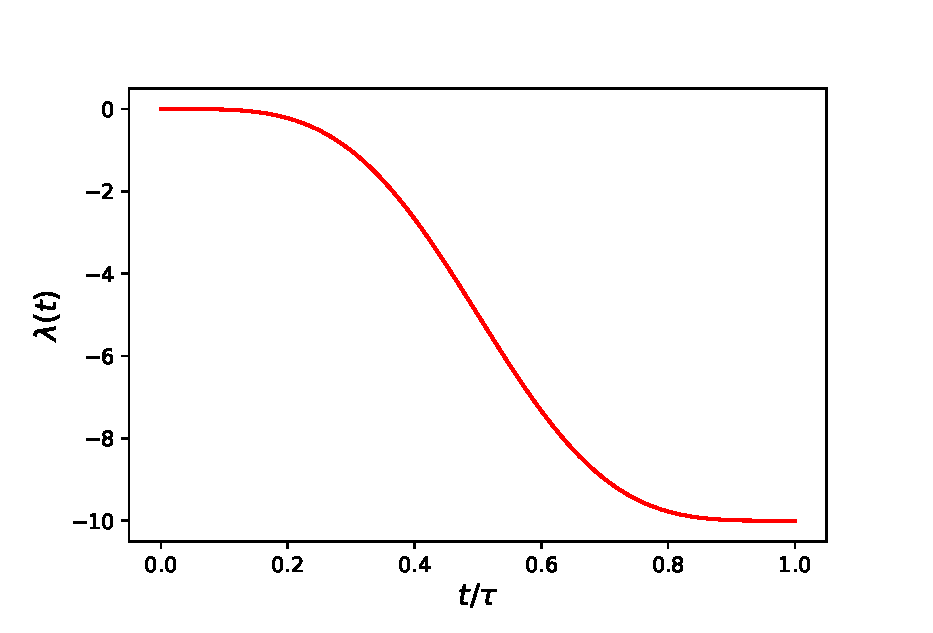
\includegraphics[scale=0.67]{protocol.eps}
\caption{Protocol chosen for going from $\lambda_i=0$ to $\lambda_f=-10J$ in time $\tau$}
\label{protocol_figure}
\end{figure}

The \textit{naive} way to drive our system will be take just our bare Hamiltonian $H_b$ and see the performance by computing $F^2$ and $E-E_0$ as we change duration of protocol $\tau$. This is shown in blue line of figure \ref{fid_energ}. We note that increasing $\tau$ improves our performance no matter how we drive our system because we are going towards adiabatic limit.


For our $\lambda$ - dependent  Hamiltonian $H_0$, approximate gauge potential is chosen to be 
\begin{equation}
A_{\lambda}^*= \sum_j \alpha_j \sigma_j^y
\end{equation}
where $\alpha_j$ are found using variational approach given in \cite{sels2017minimizing}. They find that $\alpha_j$ for $H_0$ is given by 
\begin{equation}
\alpha_j= \dfrac{1}{2} \dfrac{Z_j X_j^{\prime}- X_j Z_j^{\prime}}{Z_j^2 + X_j^2 +2J^2}
\end{equation}
Now for our $H_b$, $\alpha_j$ is given by 
\begin{equation}
\alpha_j= \delta_{j,0} \dfrac{1}{6 + (\lambda +0.8)^2}
\end{equation}
Hence, our  Hamiltonian with gauge potential term (CD term)  will be :


\begin{eqnarray}
H_{CD}&=&H_b + \dot{\lambda} A_{\lambda}^* \\
&=&H_b + \dot{\lambda} \alpha_0 \sigma_0^y 
\end{eqnarray}

In red line of figure \ref{fid_energ}, we do find that Hamiltonian with local CD term $H_{CD}$ does indeed give a better performance by increasing fidelity $F^2$ and decreasing energy above ground state $E-E_0$ for short protocol duration $\tau$. 
In Dries's paper \cite{sels2017minimizing}, they show  similar results in their figure 4, where they have used spin chain of $L=15$.



\begin{figure}
\centering
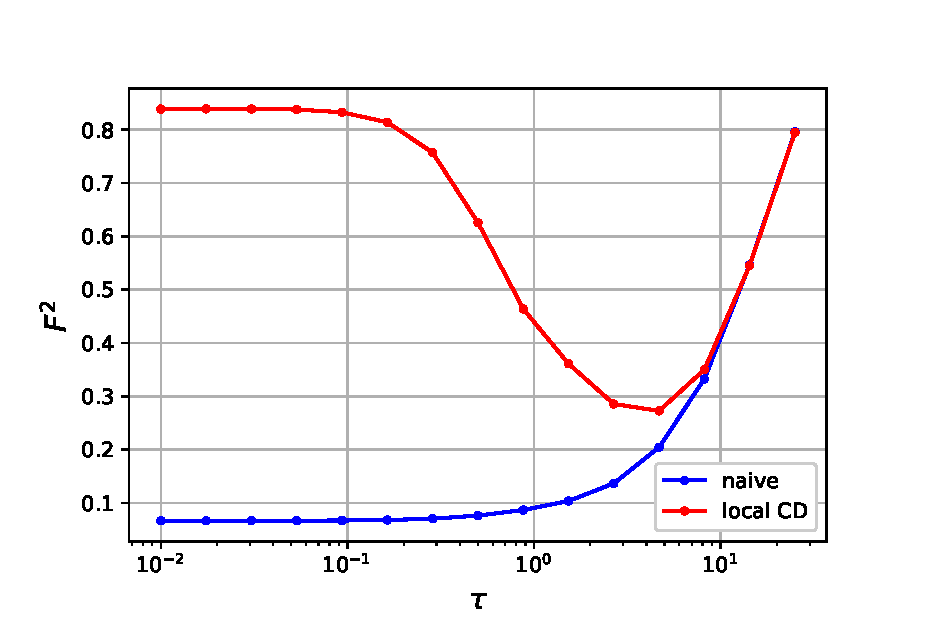
\includegraphics[scale=0.5]{fidelity_naive.eps}
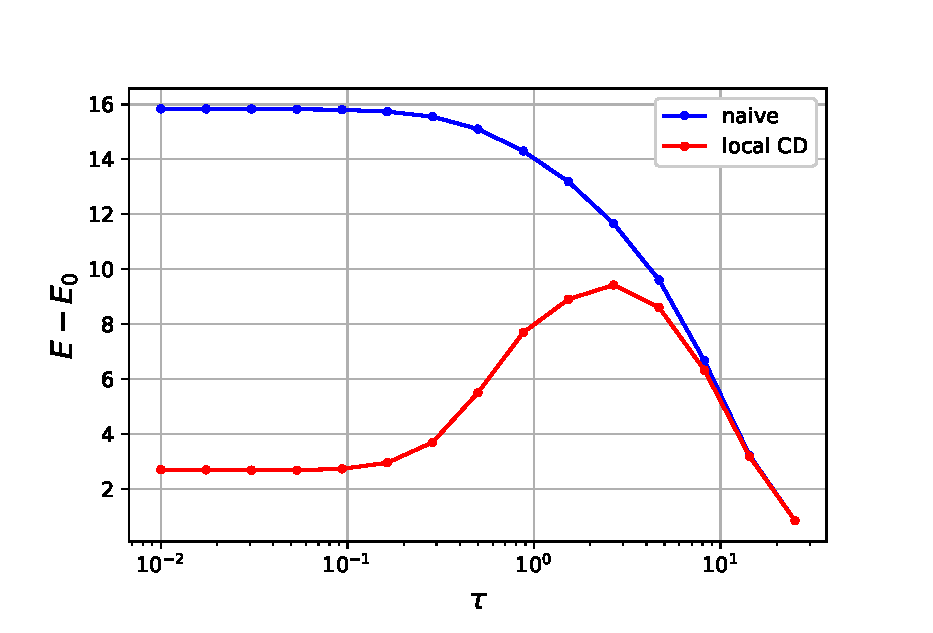
\includegraphics[scale=0.5]{final_energy_naive.eps}
\caption{Fidelity $F^2$ and final energy above ground state $E- E_0$ for L=12 spin chains}
\label{fid_energ}
\end{figure}


\section{Transverse Field Ising model: calculations in spin basis}
We would study another integrable model, which is called Transverse Field Ising model. This model shows quantum phase transition between ferromagnetic and paramagnetic phases. It's Hamiltonian is given by:
\begin{equation}
H= J \sum_{j} \sigma_j^x \sigma_{j+1}^x + h \sum_{j} \sigma_j^z + \lambda  \sigma_{0}^z
\label{xx_z_2}
\end{equation}

This model satisfies Ising symmetry $G= \Pi_i \sigma_i^z$ since $[H, G]=0$.


Since this model's exact gauge potential is already known in literature \cite{del2012assisted, kolodrubetz2016geometry}, it will be good to find either exact or approximate gauge potential using our regulator method.


Let's find out $A_{\lambda}$ for this Hamiltonian for which we need to compute different odd-powered commutator $[H, \partial_{\lambda} H]$, where $\partial_{\lambda} H=\sigma_0^z$ . Here we begin:

\begin{align}
 C^{(1)}&= -2 i J \sigma_0^y ( \sigma_{-1}^x + \sigma_1^x) \\ 
 C^{(2)}&= 8 J^2  (\sigma_0^z  +  \sigma_{-1}^x  \sigma_0^z  \sigma_1^x)- 4 J \lambda  (\sigma_{-1}^x +  \sigma_{1}^x) \sigma_0^ x  -4 h J ( (\sigma_{-1}^ x + \sigma_{1}^ x)  \sigma_0^x - (\sigma_{-1}^ y +\sigma_1^y )  \sigma_0^y ) 
 \end{align}
 
\begin{align*}
C^{(3)}= & -8 i \left(2 h^2 J \sigma _{-1}^x\sigma _{0}^y+2  h^2 J  \sigma _{-1}^y\sigma _{0}^x+2 h^2 J \sigma_{0}^x\sigma _{1}^y+   2 h^2 J \sigma _{0}^y\sigma _{1}^x-hJ^2 \sigma _{-2}^z\sigma _{-1}^z\sigma _{0}^y \right. \\
& \left. -3 h J^2 \sigma _{-1}^x\sigma_{0}^z\sigma _{1}^y-3  h J^2 \sigma _{-1}^y\sigma _{0}^z\sigma _{1}^x -hJ^2 \sigma _{0}^y\sigma _{1}^z\sigma _{2}^z \right.\\
& \left. + 2 h J \lambda\sigma _{-1}^x\sigma _{0}^y+2 h J \lambda \sigma _{-1}^y\sigma _{0}^x+2 h J \lambda\sigma _{0}^x\sigma _{1}^y+2 h J \lambda\sigma _{0}^y\sigma _{1}^x+4 J^3\sigma _{-1}^x\sigma _{0}^y \right.\\
& \left. +4 J^3\sigma_{0}^y \sigma_{1}^x+J \lambda ^2 \sigma _{-1}^x\sigma _{0}^y+J \lambda ^2\sigma _{0}^y \sigma_{1}^x \right)
\end{align*}


 
\begin{align*}
C^{(3)}= & -8 i \left(2 h^2 J (\sigma _{-1}^x+ \sigma _{1}^x)\sigma _{0}^y +2  h^2 J  (\sigma _{-1}^y + \sigma_1^y)\sigma _{0}^x -hJ^2( \sigma _{-2}^z\sigma _{-1}^z + \sigma _{1}^z\sigma _{2}^z) \sigma _{0}^y \right. \\
& \left. -3 h J^2 (\sigma _{-1}^x\sigma _{1}^y + \sigma _{-1}^y\sigma _{1}^x)\sigma _{0}^z  
 + 2 h J \lambda(\sigma _{-1}^x + \sigma _{1}^x) \sigma _{0}^y+2 h J \lambda (\sigma _{-1}^y +\sigma _{1}^y)\sigma _{0}^x  \right.\\
& \left.+ 4 J^3(\sigma _{-1}^x+ \sigma _{1}^x)\sigma _{0}^y  +J \lambda ^2(\sigma _{-1}^x+ \sigma _{1}^x)\sigma _{0}^y  \right)
\end{align*}
After rearranging terms of $(\sigma _{-1}^x+ \sigma _{1}^x)\sigma _{0}^y$, we get :


\begin{align*}
C^{(3)}= & \alpha^2 C^{(1)}-16 i   h J (h + \lambda)  (\sigma _{-1}^y + \sigma_1^y)\sigma _{0}^x + 8 i hJ^2( \sigma _{-2}^z\sigma _{-1}^z + \sigma _{1}^z\sigma _{2}^z) \sigma _{0}^y  \\
&   24 i h J^2 (\sigma _{-1}^x\sigma _{1}^y + \sigma _{-1}^y\sigma _{1}^x)\sigma _{0}^z  
\end{align*}
where $\alpha^2 =4 (4 J^2 + 2 h^2 + \lambda^2 + 2 h \lambda)= (4 J^2 +  h^2 + (h + \lambda)^2 )$

\bibliography{ref} 

\bibliographystyle{unsrt}


\end{document}